\documentclass{article}

\usepackage{fancyhdr}
\usepackage{extramarks}
\usepackage{amsmath}
\usepackage{amsthm}
\usepackage{amsfonts}
\usepackage{tikz}
\usepackage{algorithm}
\usepackage{algpseudocode}
\usepackage{enumerate}
\usepackage{tikz}
\usepackage{dsfont}
\usepackage{booktabs, multirow, array} % draw tables
\usepackage{hyperref}
\usepackage{colortbl} % cellcolor
\usetikzlibrary{arrows,automata,positioning}

%
% Basic Document Settings
%

\topmargin=-0.45in
\evensidemargin=0in
\oddsidemargin=0in
\textwidth=6.5in
\textheight=9.0in
\headsep=0.25in

\linespread{1.1}

\pagestyle{fancy}
\lhead{\hmwkAuthorName}
\chead{\hmwkClass : \hmwkTitle}
\rhead{\firstxmark}
\lfoot{\lastxmark}
\cfoot{\thepage}

\renewcommand\headrulewidth{0.4pt}
\renewcommand\footrulewidth{0.4pt}

\setlength\parindent{0pt}

%
% Create Problem Sections
%

\newcommand{\enterProblemHeader}[1]{
    \nobreak\extramarks{}{Problem \arabic{#1} continued on next page\ldots}\nobreak{}
    \nobreak\extramarks{Problem \arabic{#1} (continued)}{Problem \arabic{#1} continued on next page\ldots}\nobreak{}
}

\newcommand{\exitProblemHeader}[1]{
    \nobreak\extramarks{Problem \arabic{#1} (continued)}{Problem \arabic{#1} continued on next page\ldots}\nobreak{}
    \stepcounter{#1}
    \nobreak\extramarks{Problem \arabic{#1}}{}\nobreak{}
}

\newcommand*\circled[1]{\tikz[baseline=(char.base)]{
		\node[shape=circle,draw,inner sep=2pt] (char) {#1};}}


\setcounter{secnumdepth}{0}
\newcounter{partCounter}
\newcounter{homeworkProblemCounter}
\setcounter{homeworkProblemCounter}{1}
\nobreak\extramarks{Problem \arabic{homeworkProblemCounter}}{}\nobreak{}

%
% Homework Problem Environment
%
% This environment takes an optional argument. When given, it will adjust the
% problem counter. This is useful for when the problems given for your
% assignment aren't sequential. See the last 3 problems of this template for an
% example.
%

\newenvironment{homeworkProblem}[1][-1]{
    \ifnum#1>0
        \setcounter{homeworkProblemCounter}{#1}
    \fi
    \section{Problem \arabic{homeworkProblemCounter}}
    \setcounter{partCounter}{1}
    \enterProblemHeader{homeworkProblemCounter}
}{
    \exitProblemHeader{homeworkProblemCounter}
}

%
% Homework Details
%   - Title
%   - Class
%   - Due date
%   - Name
%   - Student ID

\newcommand{\hmwkTitle}{Homework\ \#06}
\newcommand{\hmwkClass}{SI252 Reinforcement Learning}
\newcommand{\hmwkDueDate}{June 1, 2025}
\newcommand{\hmwkAuthorName}{Zhou Shouchen}
\newcommand{\hmwkAuthorID}{2021533042}


%
% Title Page
%

\title{
    \vspace{2in}
    \textmd{\textbf{\hmwkClass:\\  \hmwkTitle}} \\
    \normalsize\vspace{0.1in}\small{Due\ on\ \hmwkDueDate\ at 11:59 p.m.(CST)} \\
	\vspace{4in}
}

\author{
	Name: \textbf{\hmwkAuthorName} \\
	Student ID: \hmwkAuthorID}
\date{}

\renewcommand{\part}[1]{\textbf{\large Part \Alph{partCounter}}\stepcounter{partCounter}\\}

%
% Various Helper Commands
%

% Useful for algorithms
\newcommand{\alg}[1]{\textsc{\bfseries \footnotesize #1}}
% For derivatives
\newcommand{\deriv}[1]{\dfrac{\mathrm{d}}{\mathrm{d}x} (#1)}
% For partial derivatives
\newcommand{\pderiv}[2]{\dfrac{\partial}{\partial #1} (#2)}
% Integral dx
\newcommand{\dx}{\mathrm{d}x}
\newcommand{\dt}{\mathrm{d}t}
\newcommand{\du}{\mathrm{d}u}
\newcommand{\dr}{\mathrm{d}r}
\newcommand{\dS}{\mathrm{d}S}
\newcommand{\dtheta}{\mathrm{d}\theta}
\newcommand{\dphi}{\mathrm{d}\phi}
\newcommand{\domega}{\mathrm{d}\omega}
\newcommand{\dU}{\mathrm{d}U}
\newcommand{\dV}{\mathrm{d}V}


% Alias for the Solution section header
\newcommand{\solution}{\textcolor{blue}{\textbf{Solution}}}
% Probability commands: Expectation, Variance, Covariance, Bias
\newcommand{\E}{\mathbb{E}}
\newcommand{\Var}{\mathrm{Var}}
\newcommand{\Cov}{\mathrm{Cov}}
\newcommand{\Bias}{\mathrm{Bias}}
\newcommand{\Unif}{\operatorname{Unif}}
\newcommand{\Beta}{\operatorname{Beta}}
\newcommand{\Bin}{\operatorname{Bin}}
\newcommand{\Bern}{\operatorname{Bern}}
\newcommand{\Expo}{\operatorname{Expo}}
\newcommand{\FS}{\operatorname{FS}}
\newcommand{\Pois}{\operatorname{Pois}}
\newcommand{\N}{\mathcal{N}}
\newcommand{\A}{\mathcal{A}}
\newcommand{\mS}{\mathcal{S}}
\newcommand{\R}{\mathcal{R}}
\newcommand{\mP}{\mathcal{P}}
\newcommand{\I}{\mathbb{I}}
\newcommand{\indep}{\perp \!\!\! \perp} % independent symbol
\newcommand{\argmin}{\mathop{\rm argmin}}
\newcommand{\argmax}{\mathop{\rm argmax}}
\newcommand{\sgn}{\operatorname{sgn}}
\newcommand{\bpi}{\boldsymbol{\pi}}
\newcommand{\cnt}{\text{count}}

\newcommand{\bmu}{\boldsymbol{\mu}}
\newcommand{\bSigma}{\boldsymbol{\Sigma}}
\newcommand{\diag}{\operatorname{diag}}



\begin{document}

\maketitle
\pagebreak

\begin{homeworkProblem}

\textbf{Required: OpenAI Spinning Up in Deep RL}. Welcome to \href{https://spinningup.openai.com/en/latest/user/introduction.html}{Spinning Up in Deep RL}! This is an educational resource produced by OpenAI that makes it easier to learn about deep reinforcement learning (deep RL). Please study the documents and install the environment with PyTorch version.

(a) Finish the problem set 1: ``\href{https://spinningup.openai.com/en/latest/spinningup/exercises.html#problem-set-1-basics-of-implementation}{Basics of Implementation}". It includes three exercises: Gaussian Log-Likelihood, Policy for PPO, and Computation Graph for TD3.

(b) Finish the problem set 2: ``\href{https://spinningup.openai.com/en/latest/spinningup/exercises.html#problem-set-2-algorithm-failure-modes}{Algorithm Failure Modes}". It includes two exercises: Value Function Fitting in TRPO, and Silent Bug in DDPG.

\solution

(a) After setting up the environment in the methods in `README.md', we can successfully run the codes. The codes cuold be check in `code/spinningup/spinup/exercises/pytorch/problem\_set\_1'.

\begin{itemize}
    \item exercise 1\_1: For a $k$ dimension diagnoal Gaussian distribtion $\mathbf{x}\sim\N(\bmu,\bSigma)$, where $\bSigma=\diag(\sigma_1^2,\dots,\sigma_k^2)$, thus its PDF is
    $$p(\mathbf{x};\bmu,\bSigma)=\dfrac{1}{(2\pi)^{\frac{k}{2}}\,|\bSigma|^{\frac{1}{2}}}\exp\left[-\frac{1}{2}(\mathbf{x}-\bmu)^{\top}\bSigma^{-1}(\mathbf{x}\bmu)\right]$$
    Where
    $$|\bSigma|=\prod_{i=1}^{k}\sigma_i^{2}, \qquad \bSigma^{-1}=\diag\left(\sigma_1^{-2},\dots,\sigma_k^{-2}\right), \qquad (\mathbf{x}-\bmu)^{\top}\bSigma^{-1}(\mathbf{x}-\bmu)=\sum_{i=1}^{k}\frac{(x_i-\mu_i)^2}{\sigma_i^{2}}$$
    So above all, the log-likelihood is
    \begin{align*}
    \log p(\mathbf{x};\bmu,\bSigma) &= -\frac{k}{2}\log(2\pi)-\sum_{i=1}^{k}\log\sigma_i-\frac{1}{2}\sum_{i=1}^{k}\frac{(x_i-\mu_i)^2}{\sigma_i^{2}} \\
    &= -\dfrac{1}{2}\sum_{i=1}^k\left(\log(2\pi)+2\log\sigma_i+\left(\dfrac{x_i-\mu_i}{\sigma_i}\right)^2\right)
    \end{align*}

    The implementation are check results are as follows:
    \begin{figure}[h]
        \centering
        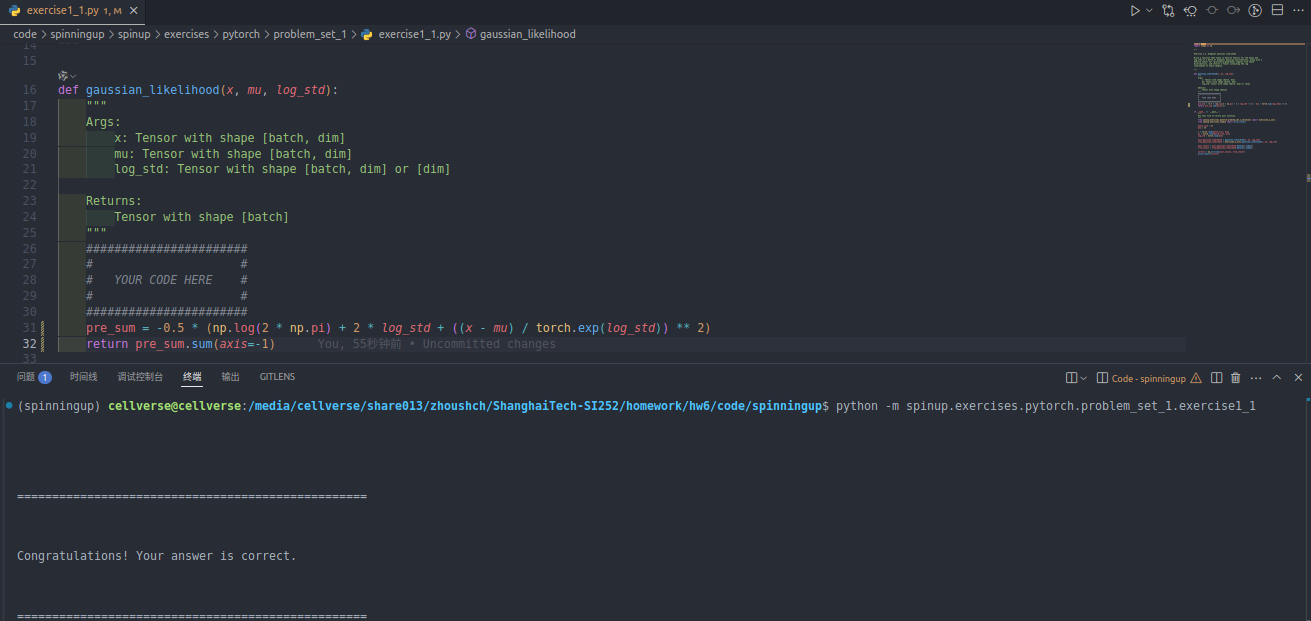
\includegraphics[width=\textwidth]{../Img/spinningup_exercises/1_1.png}
    \end{figure}

    \item exercise 1\_2: The implementation are check results are as follows:
    \begin{figure}[h]
        \centering
        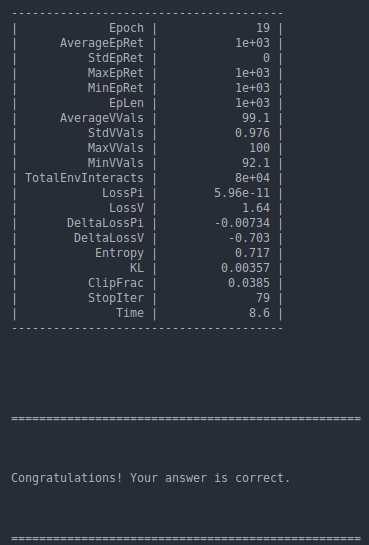
\includegraphics[width=0.5\textwidth]{../Img/spinningup_exercises/1_2.png}
    \end{figure}

    \item exercise 1\_3:
    According to the discription, within 10 rounds, the score in HalfSheetah should exceed 300, while the score in InvertedPendulum should reach 150.

    And the following curves show that the performance achieved the expected results:
    \begin{figure}[H]
        \centering
        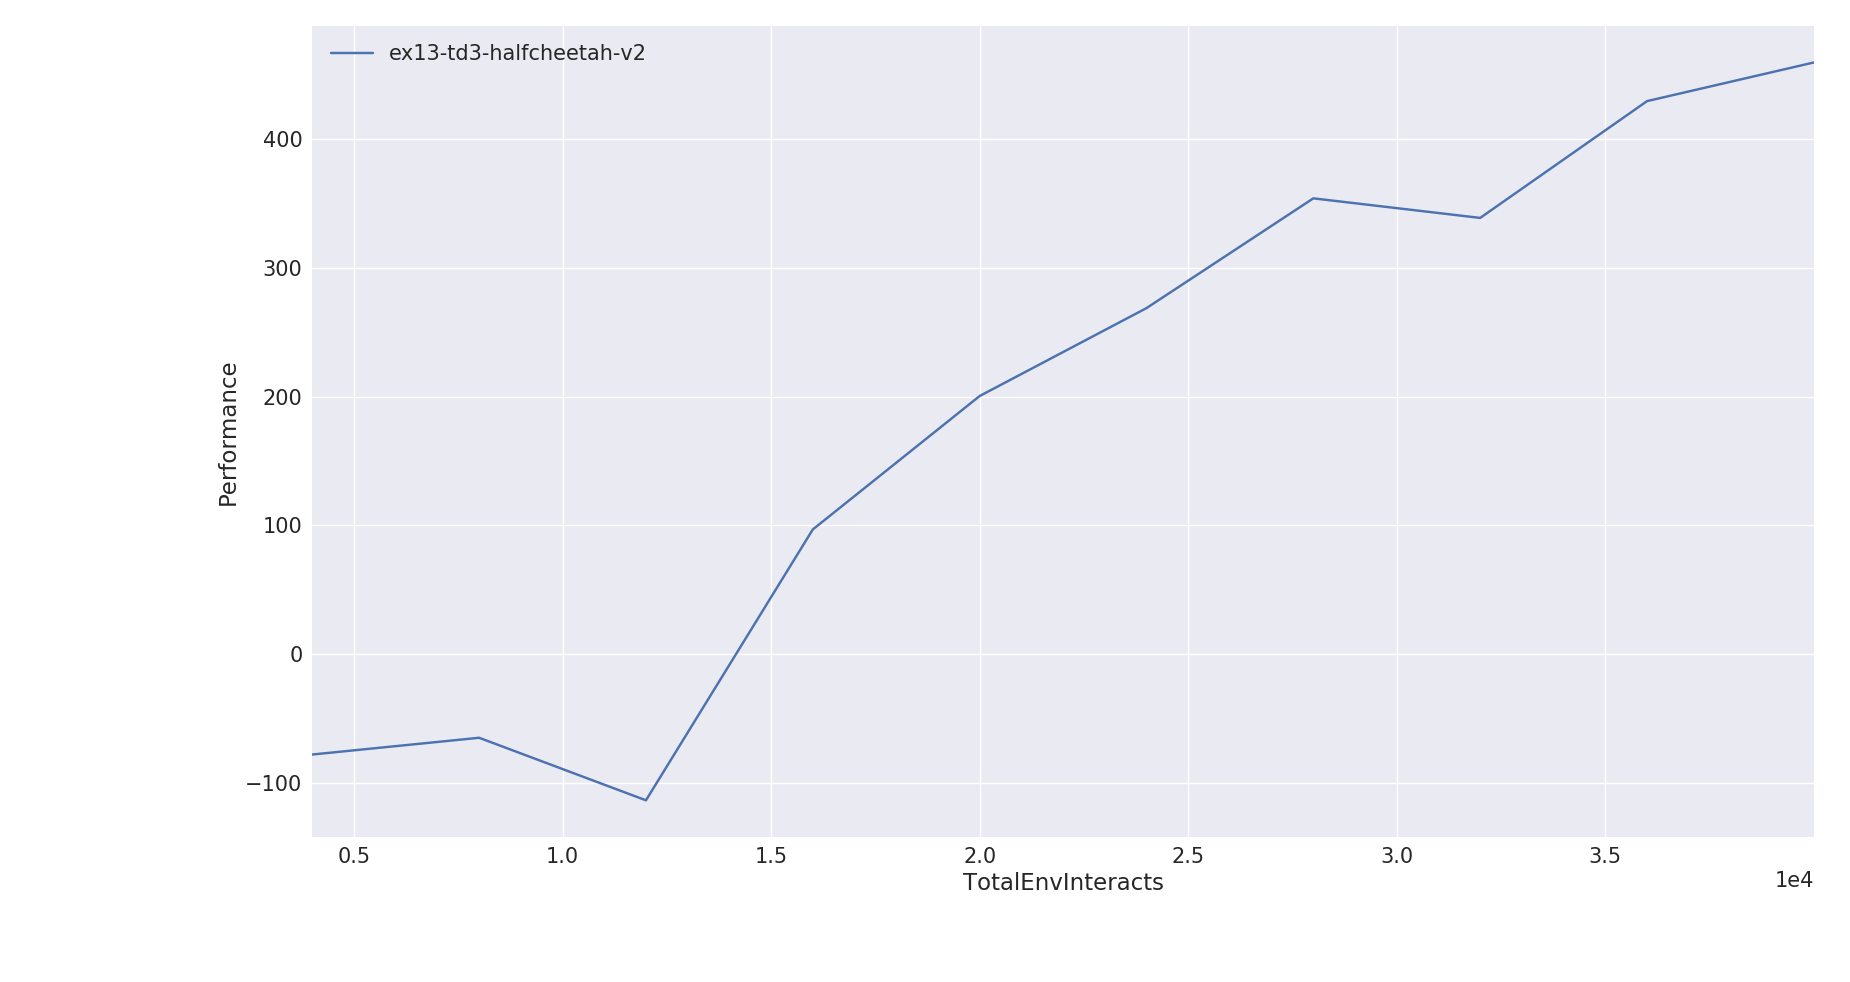
\includegraphics[width=\textwidth]{../Img/spinningup_exercises/1_3_healthcare.png}
        \vspace{-2cm}
    \end{figure}
    \begin{figure}[H]
        \centering
        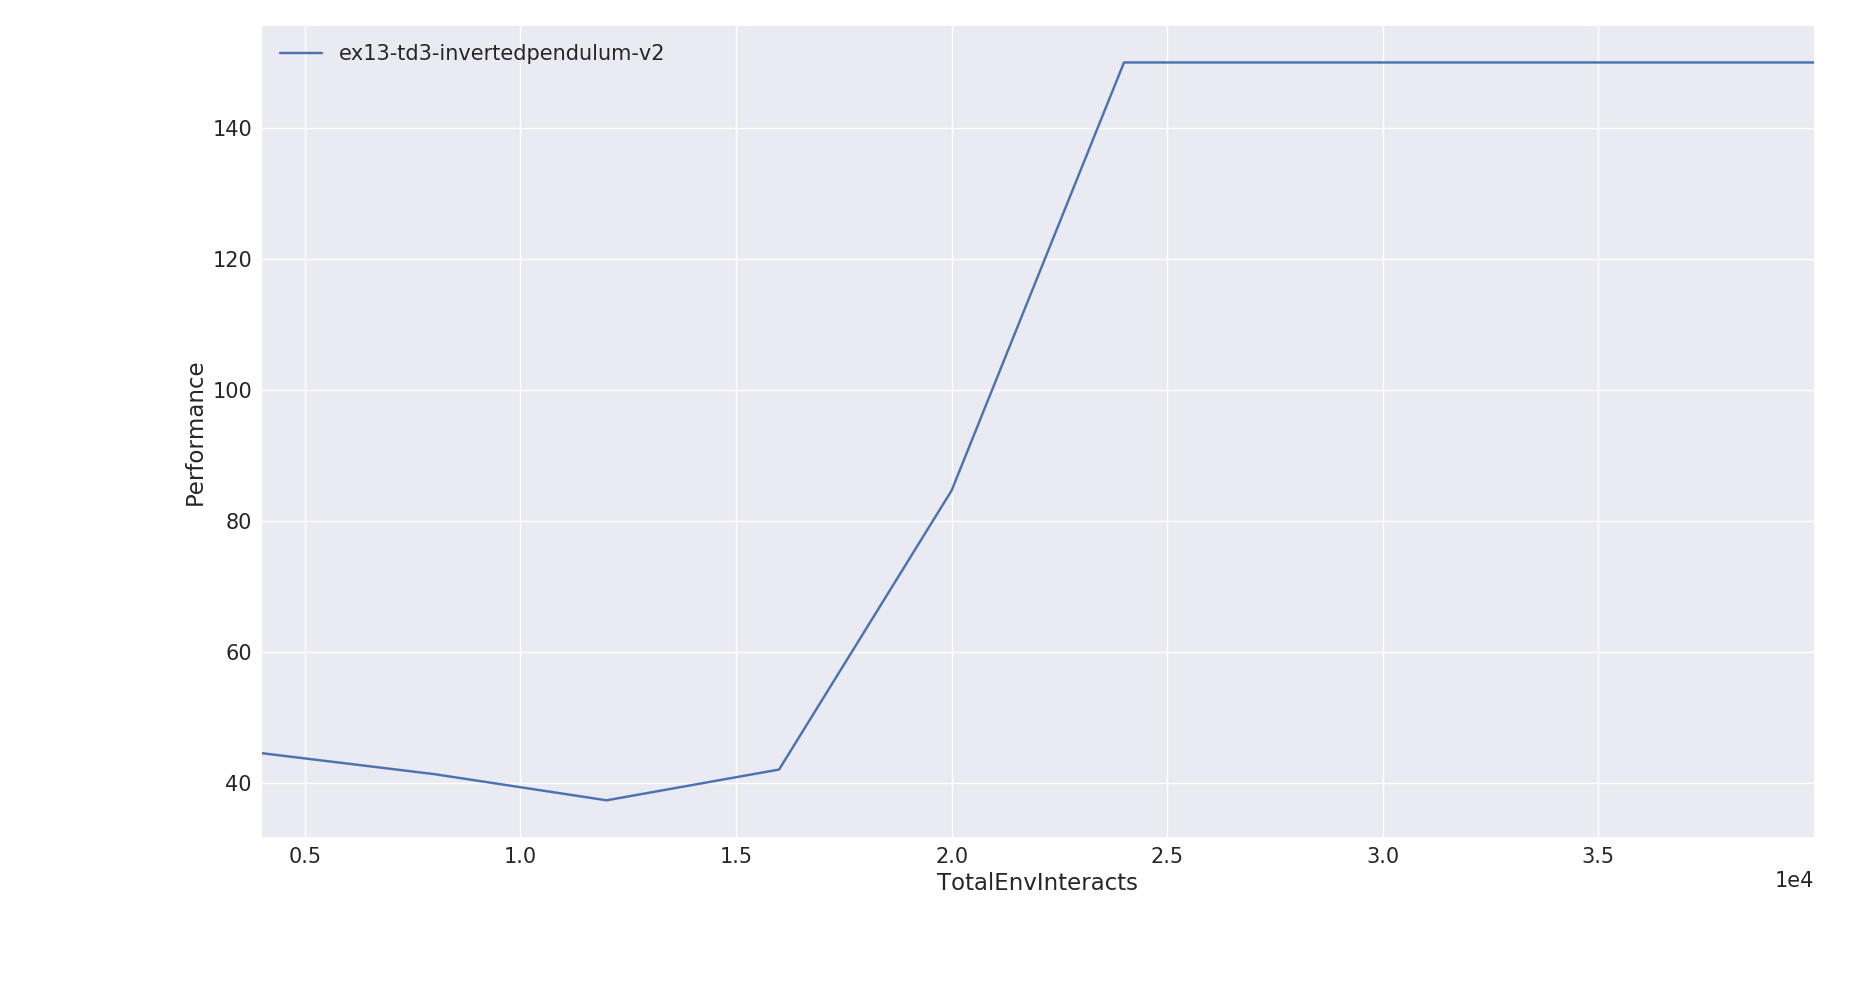
\includegraphics[width=\textwidth]{../Img/spinningup_exercises/1_3_invertedpendulum.png}
    \end{figure}

\end{itemize}


(b) Run the commands in the `README.md', we can get the following reults. The codes cuold be check in `code/spinningup/spinup/exercises/pytorch/problem\_set\_2'.

\begin{itemize}
    \item exercise 2\_1:

    The difference is quite substantial: with a trained value function, the agent is able to quickly make progress. With an untrained value function, the agent gets stuck early on.

    The curve of v0 with different seeds are as follows:
    \begin{figure}[H]
        \centering
        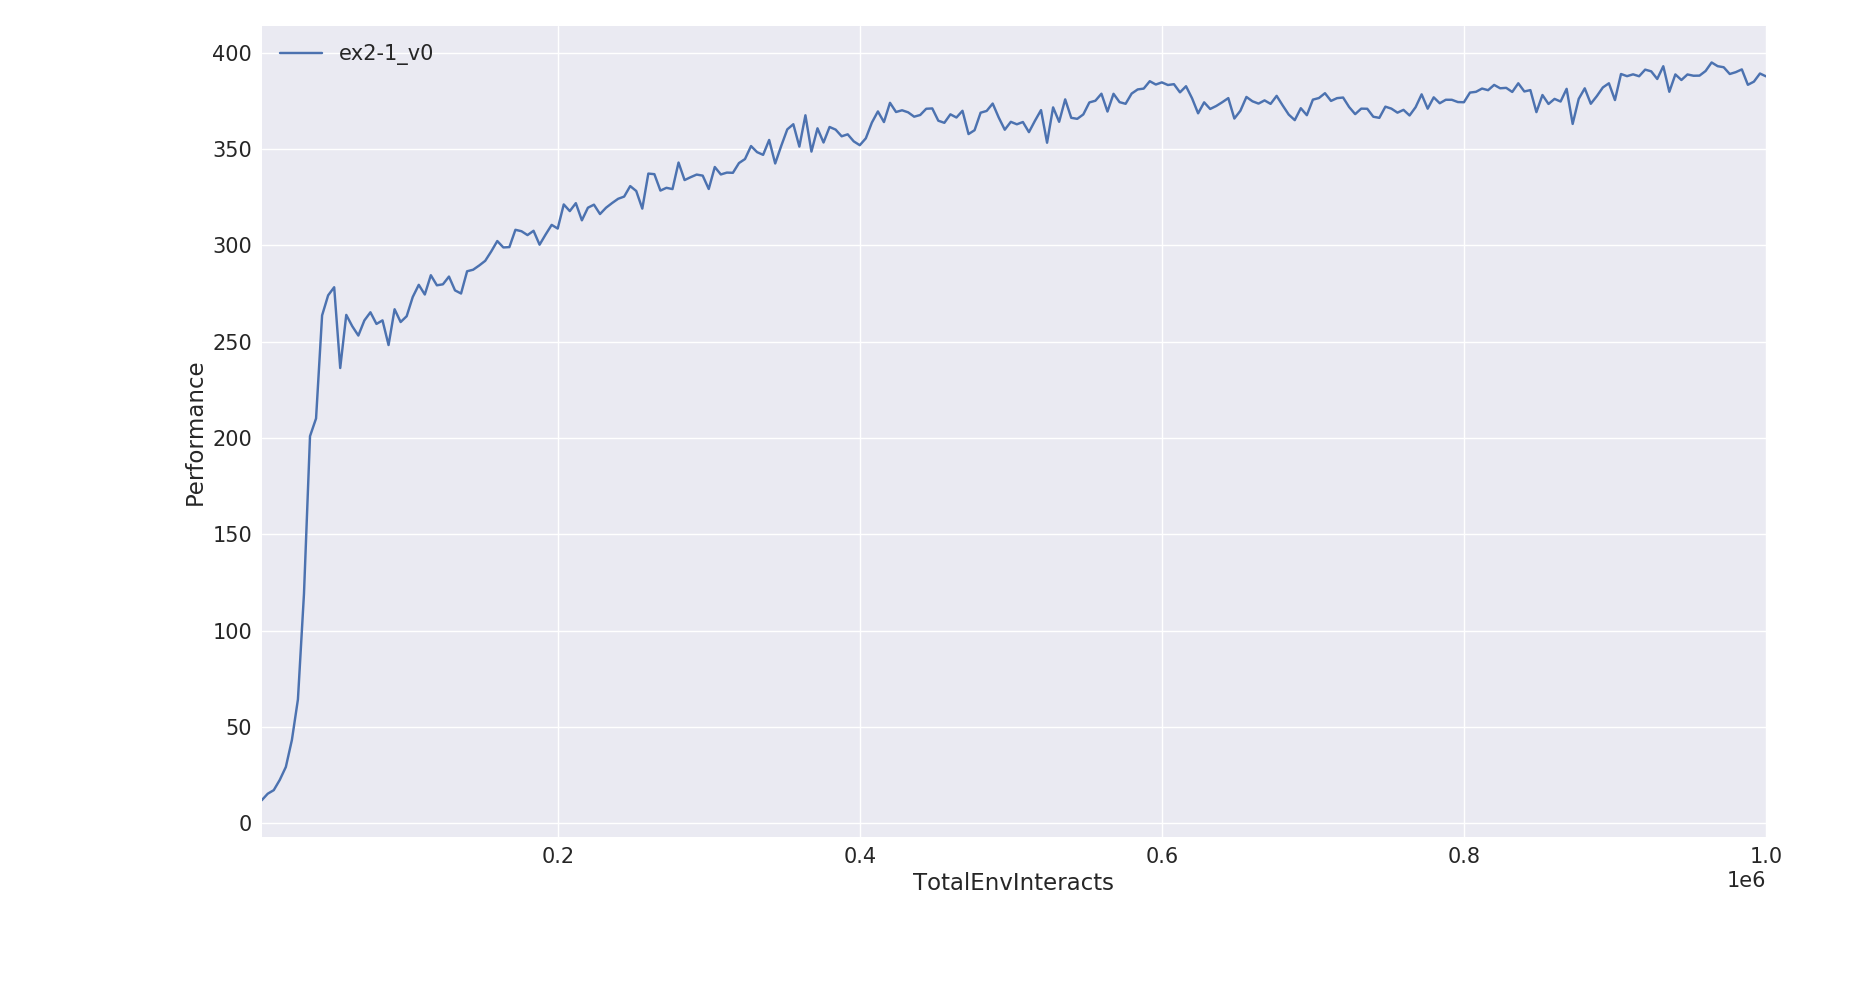
\includegraphics[width=0.32\textwidth]{../Img/spinningup_exercises/2_1/2_1_curve_v0_s0.png}
        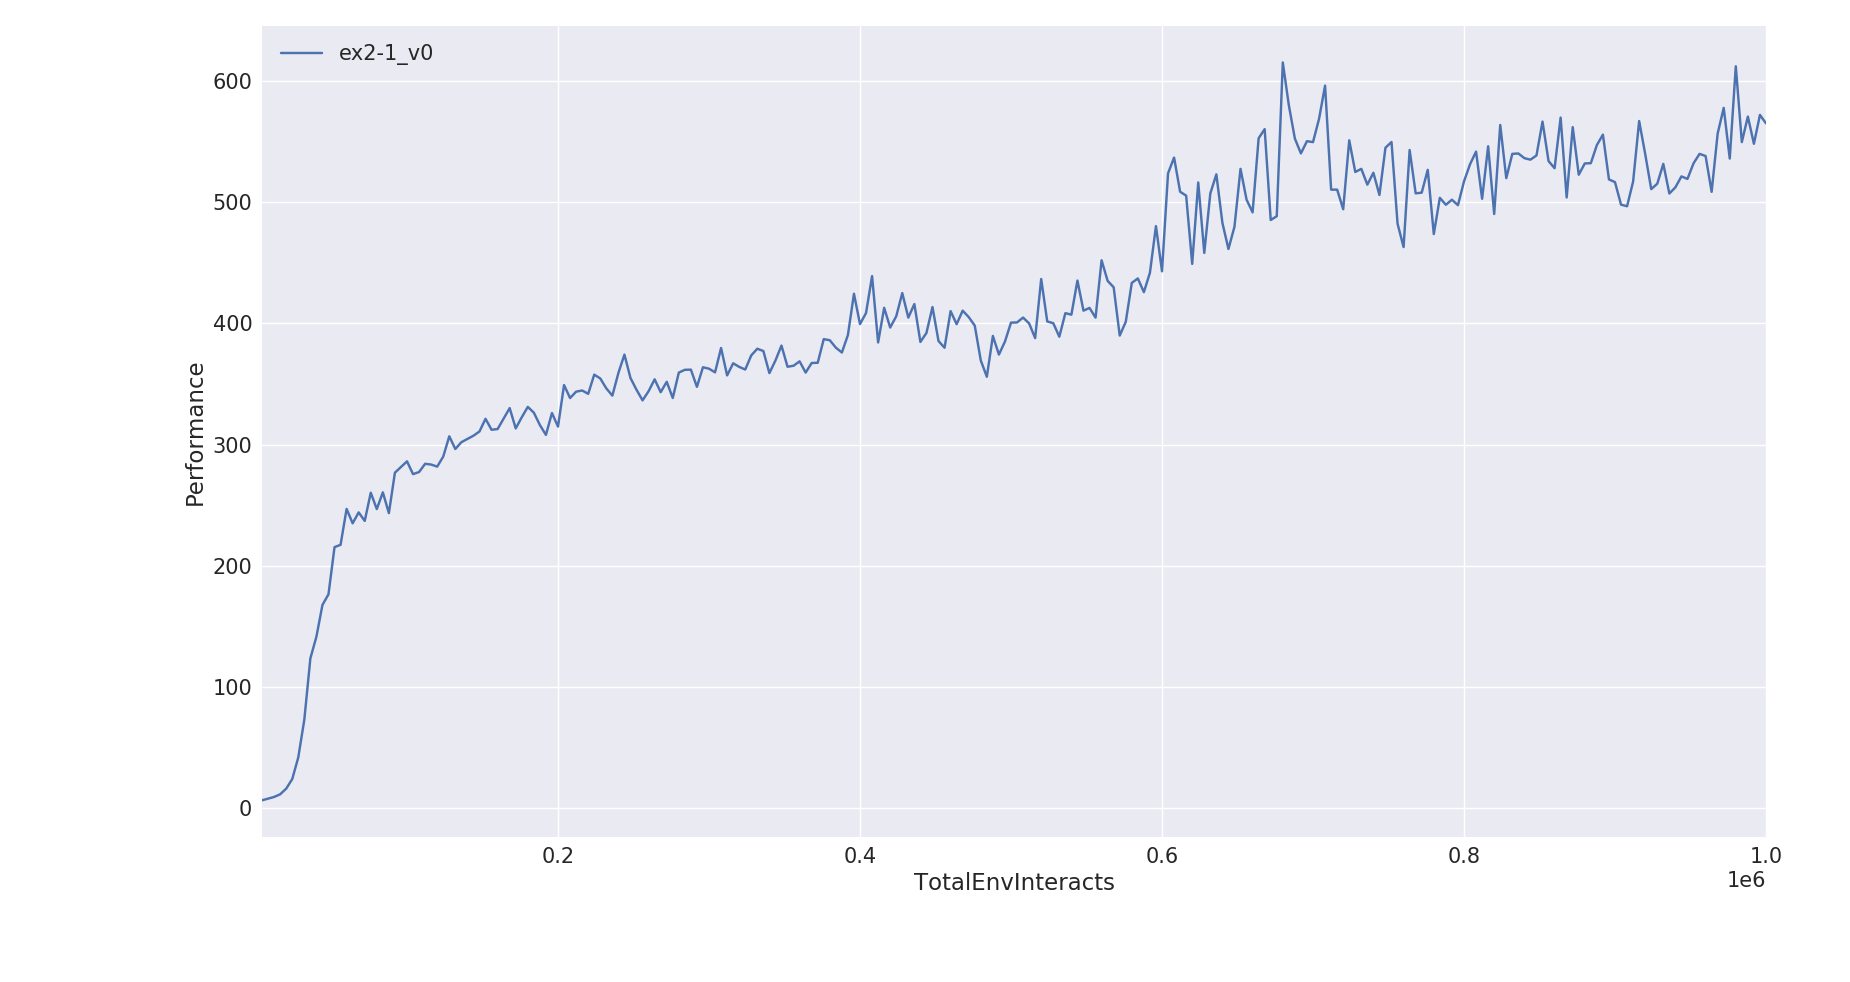
\includegraphics[width=0.32\textwidth]{../Img/spinningup_exercises/2_1/2_1_curve_v0_s10.png}
        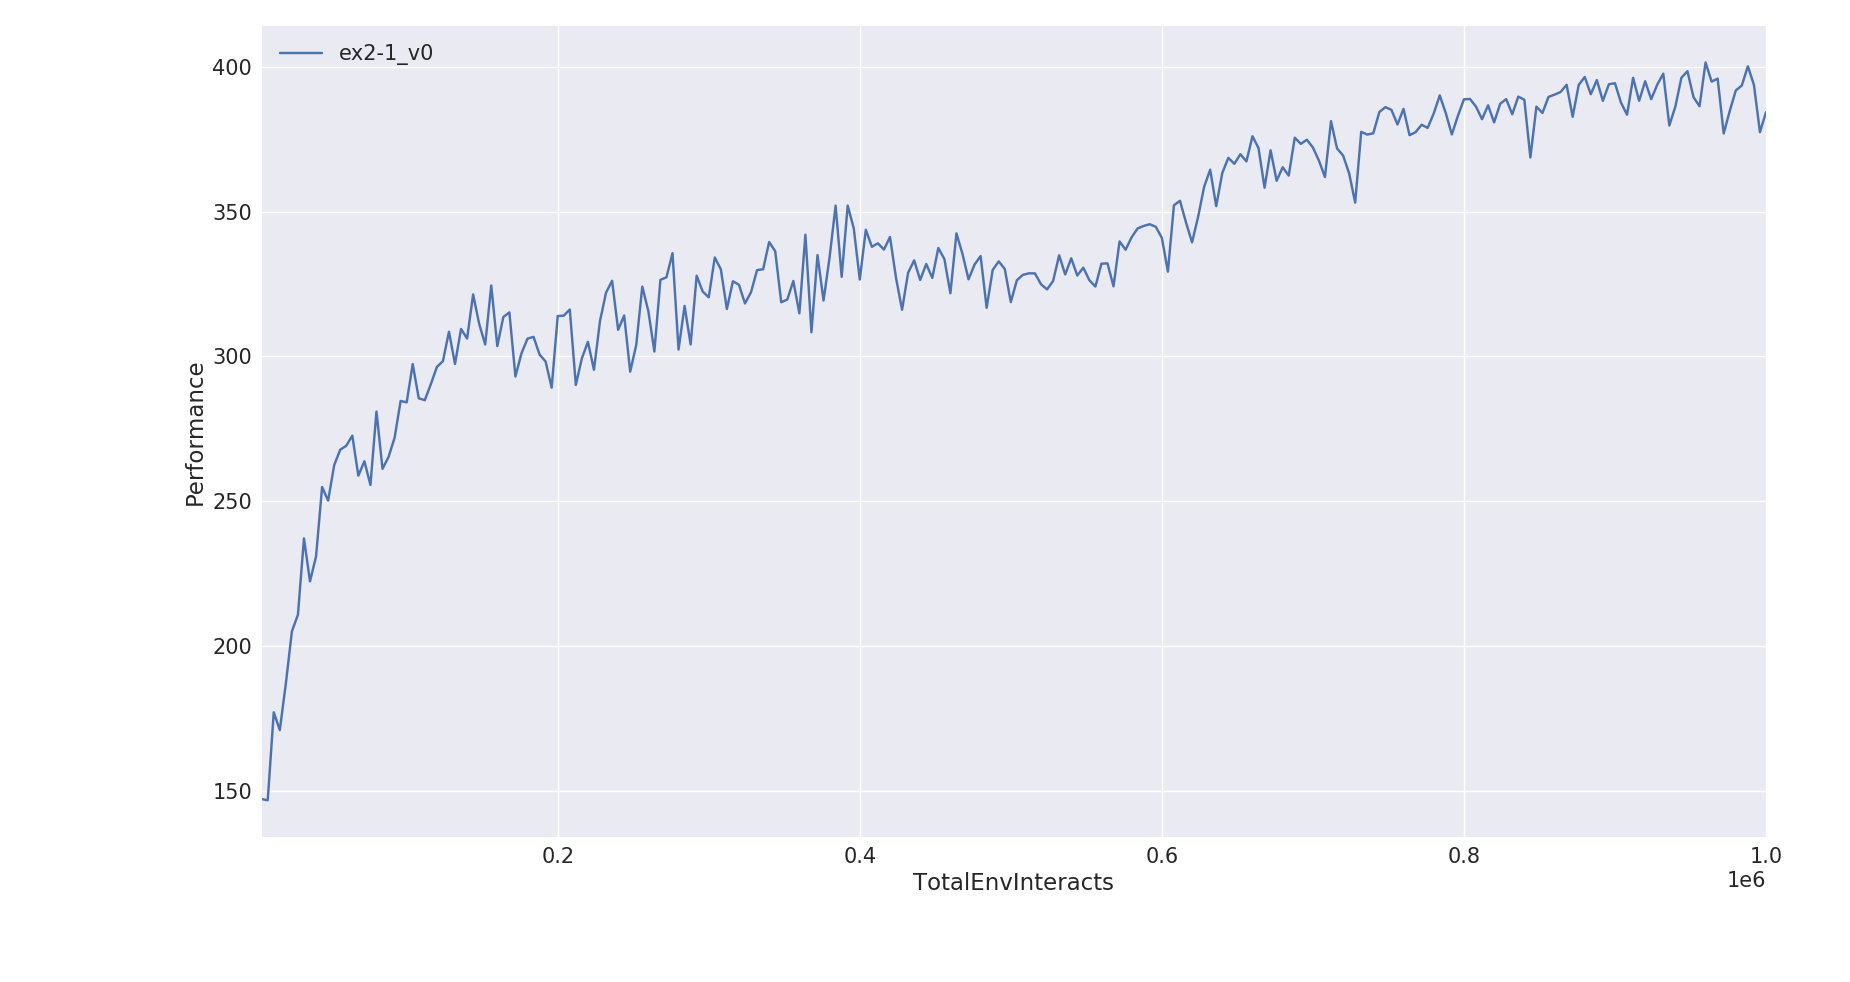
\includegraphics[width=0.32\textwidth]{../Img/spinningup_exercises/2_1/2_1_curve_v0_s20.png}
    \end{figure}

    The curve of v80 with different seeds are as follows:
    \begin{figure}[H]
        \centering
        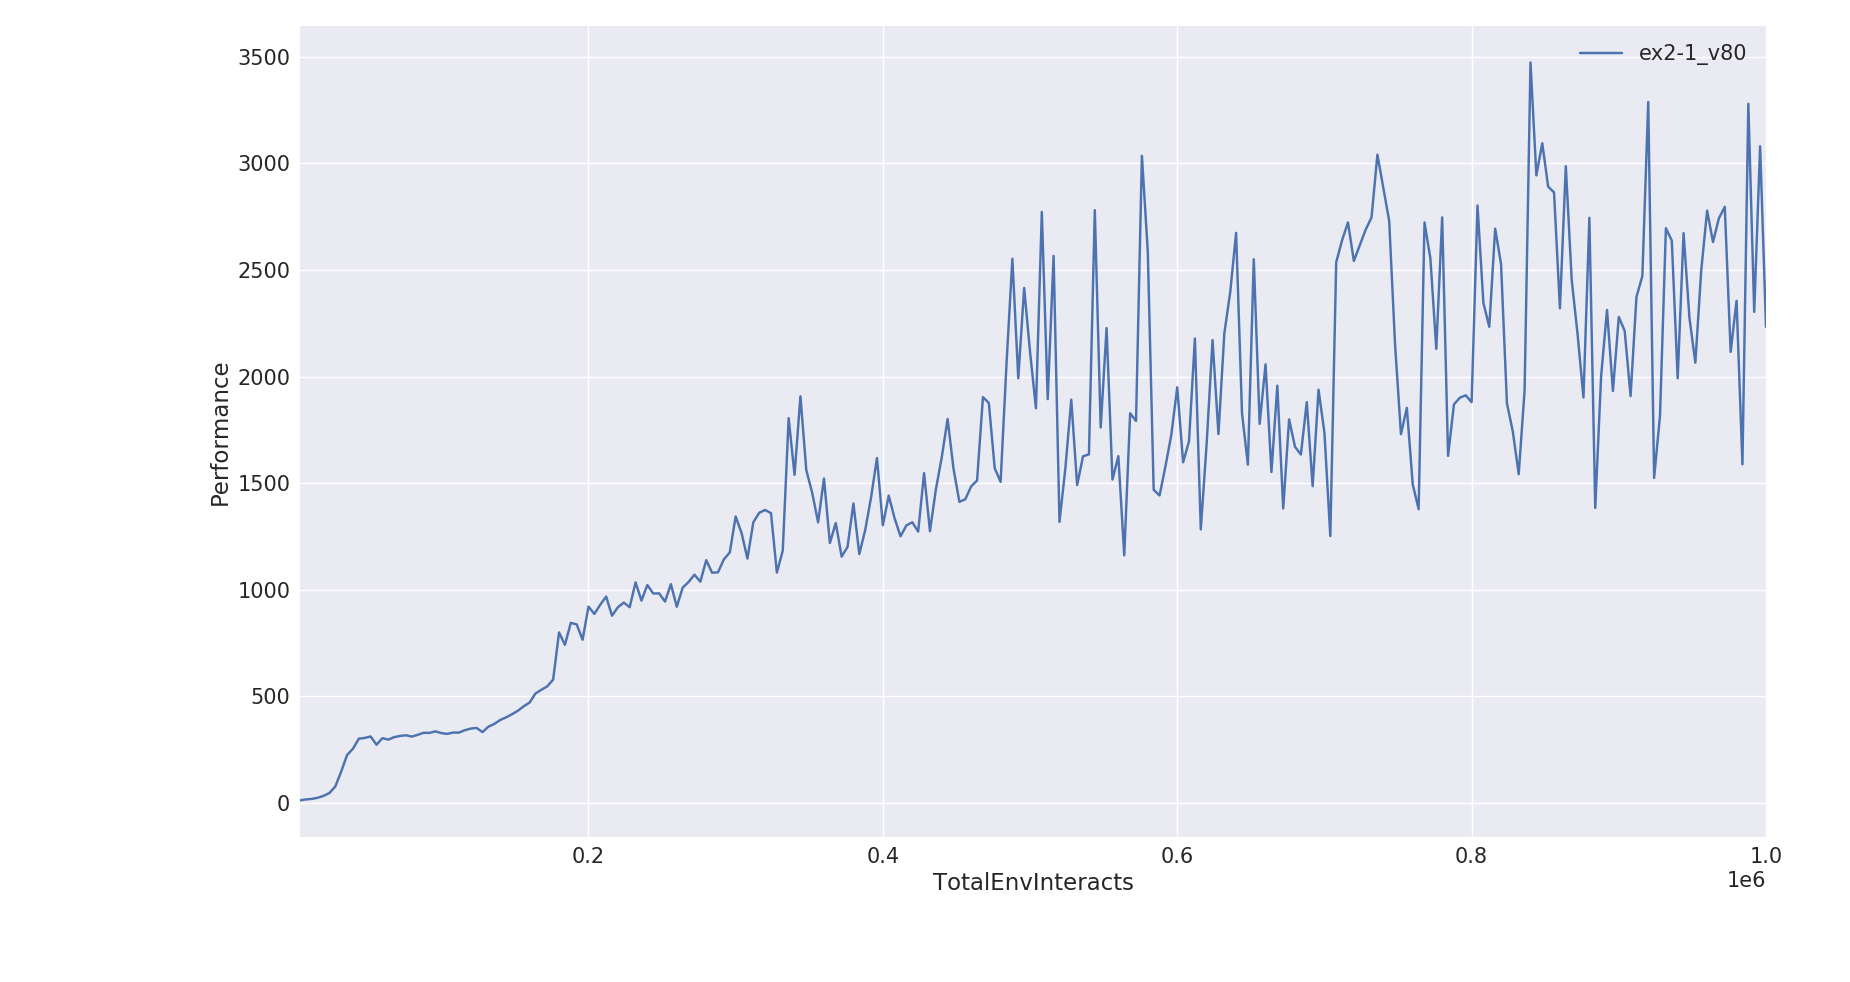
\includegraphics[width=0.32\textwidth]{../Img/spinningup_exercises/2_1/2_1_curve_v80_s0.png}
        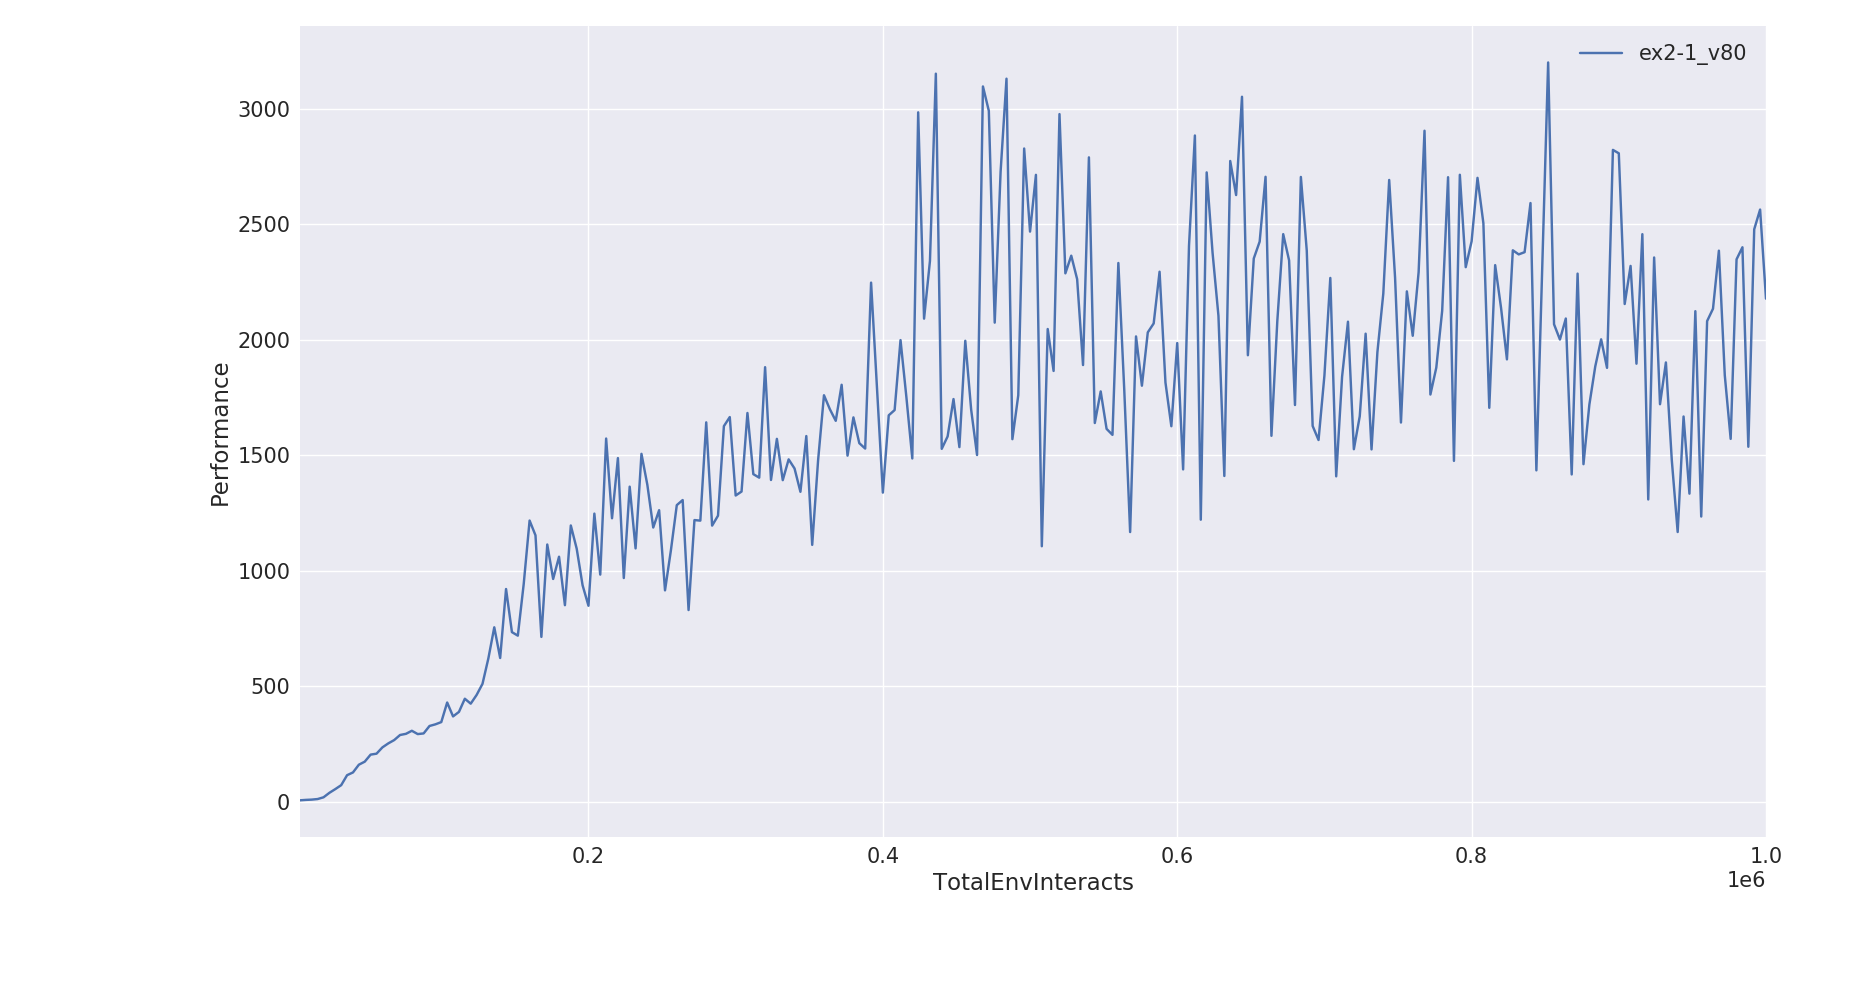
\includegraphics[width=0.32\textwidth]{../Img/spinningup_exercises/2_1/2_1_curve_v80_s10.png}
        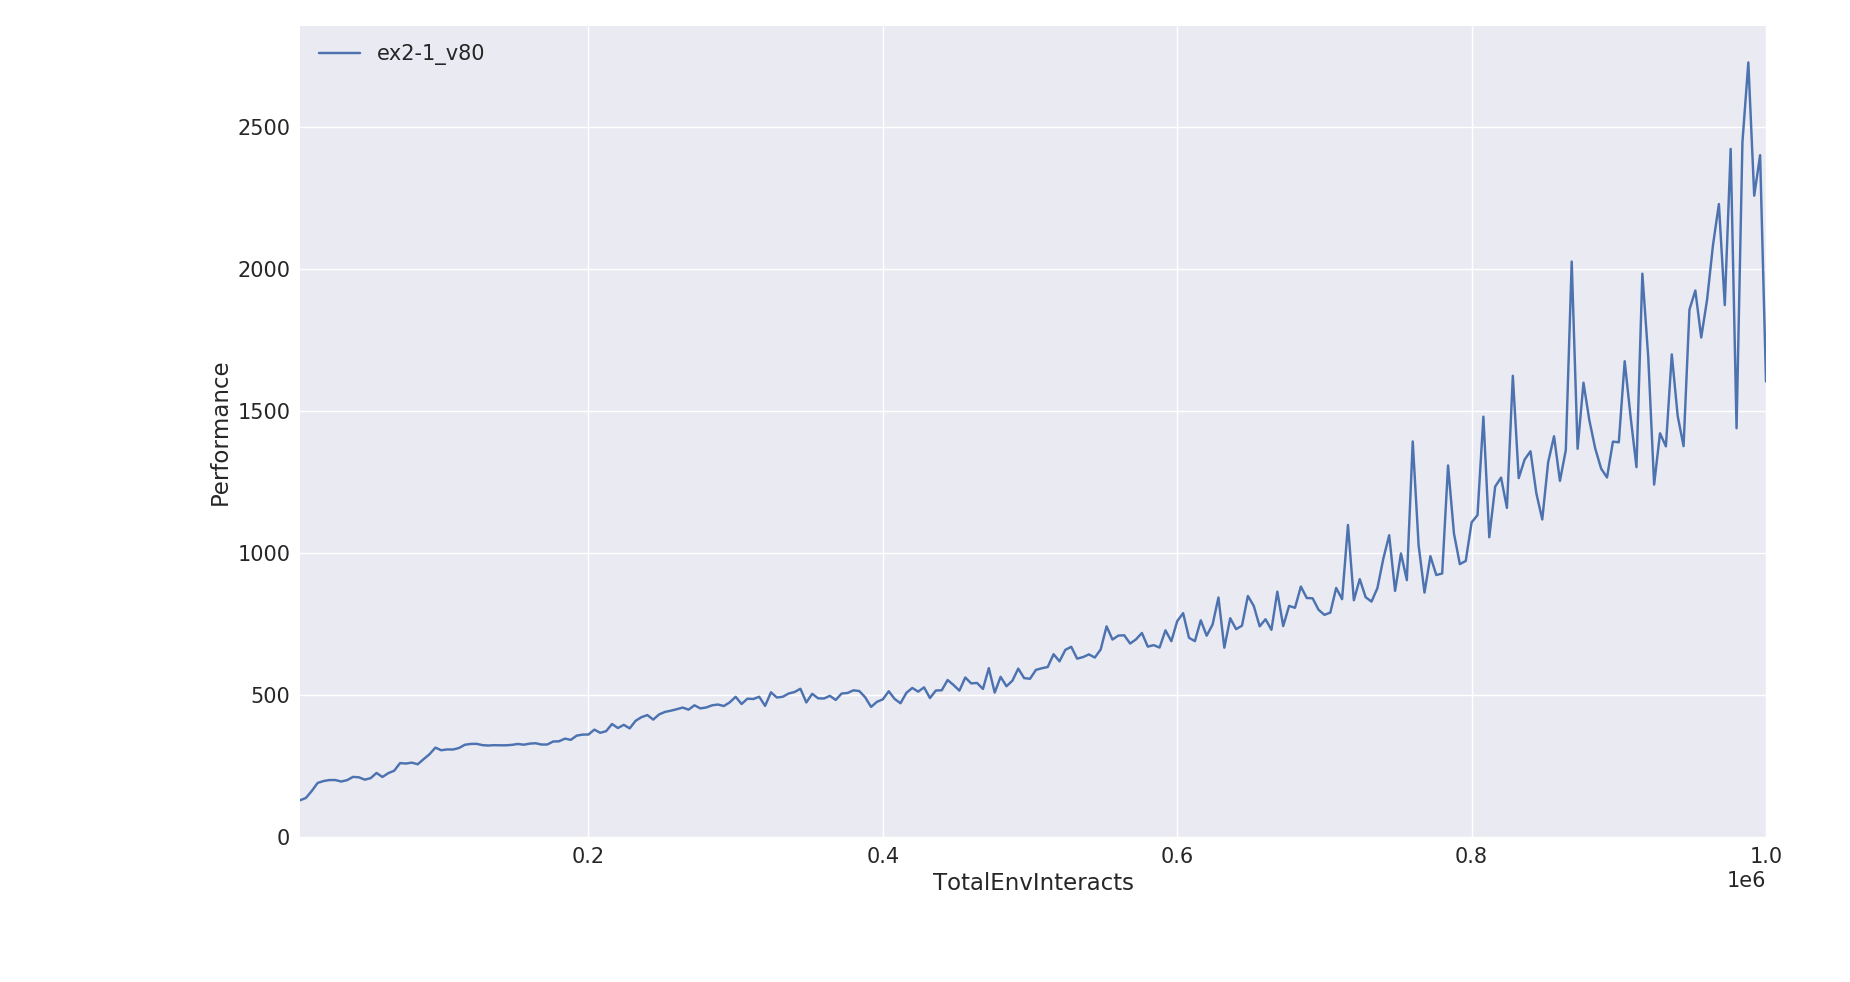
\includegraphics[width=0.32\textwidth]{../Img/spinningup_exercises/2_1/2_1_curve_v80_s20.png}
    \end{figure}

    The comparison between curve of v0 and v80, and their average and variance are as follows:
    \begin{figure}[H]
        \centering
        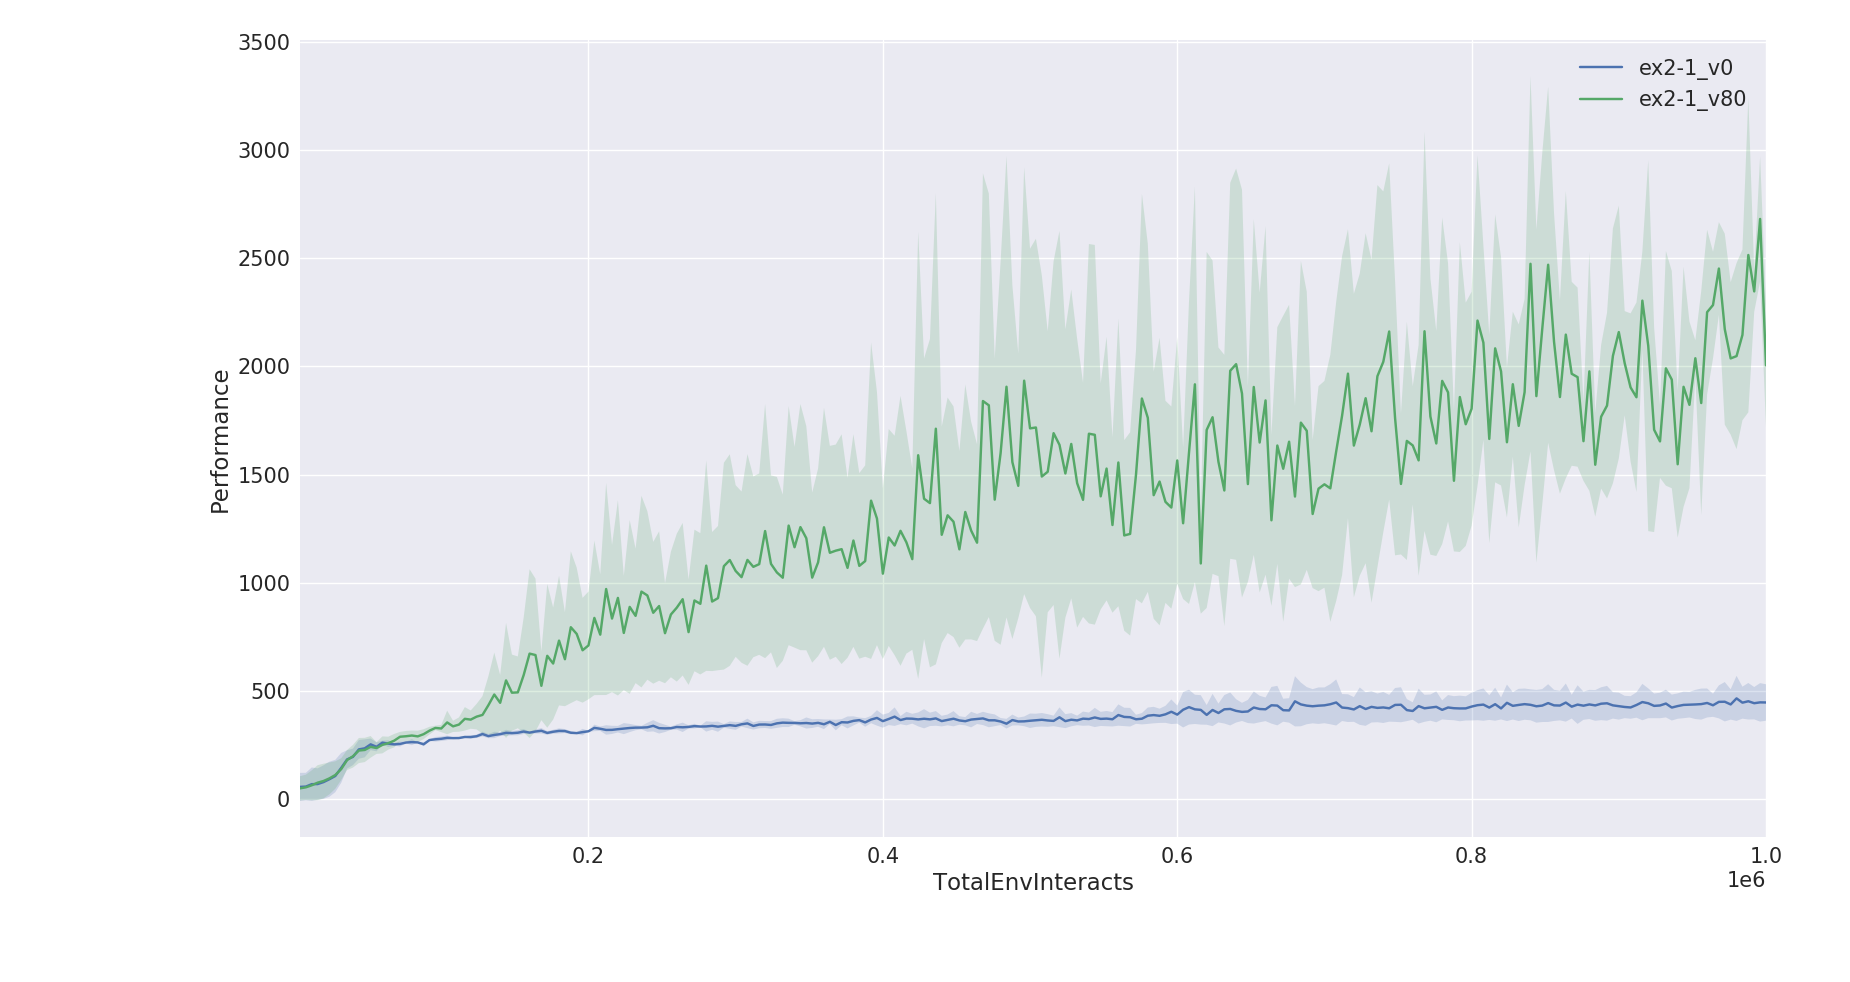
\includegraphics[width=\textwidth]{../Img/spinningup_exercises/2_1/2_1_curve_all.png}
    \end{figure}

    \item exercise 2\_2:
    The curve of the code without bug and with different seeds are as follows:
    \begin{figure}[H]
        \centering
        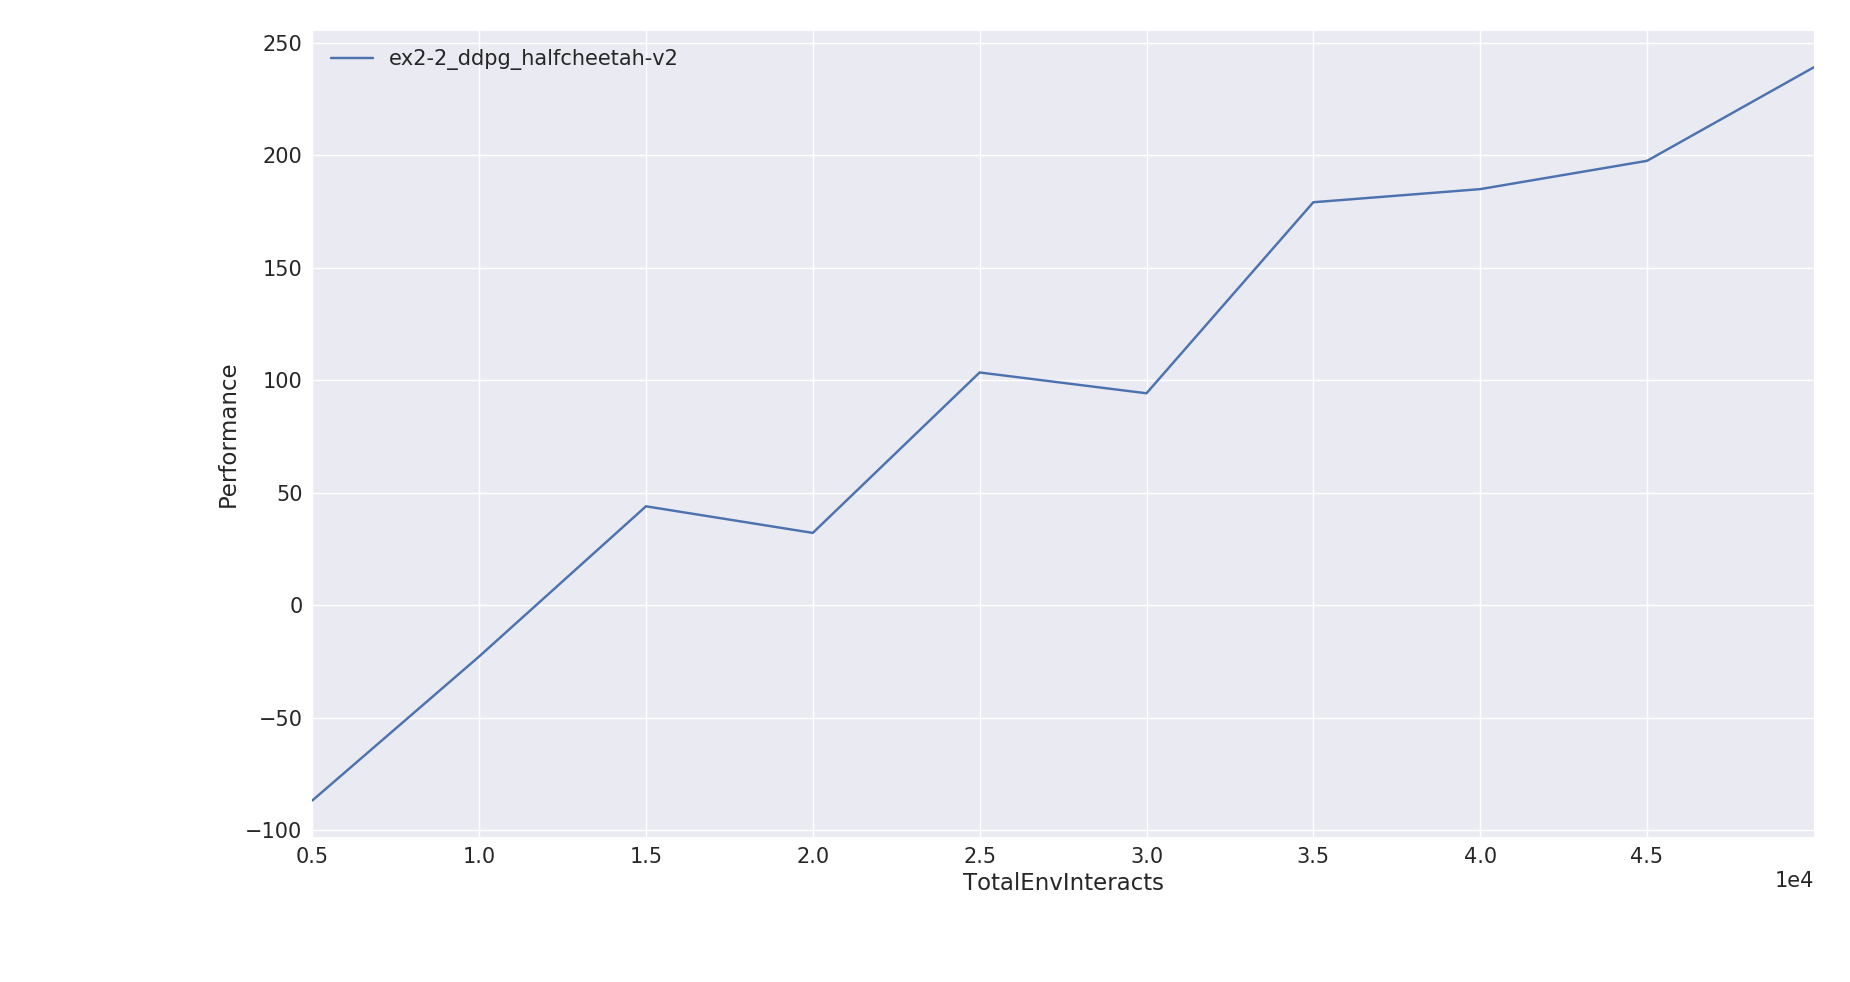
\includegraphics[width=0.32\textwidth]{../Img/spinningup_exercises/2_2/2_2_curve_s0.png}
        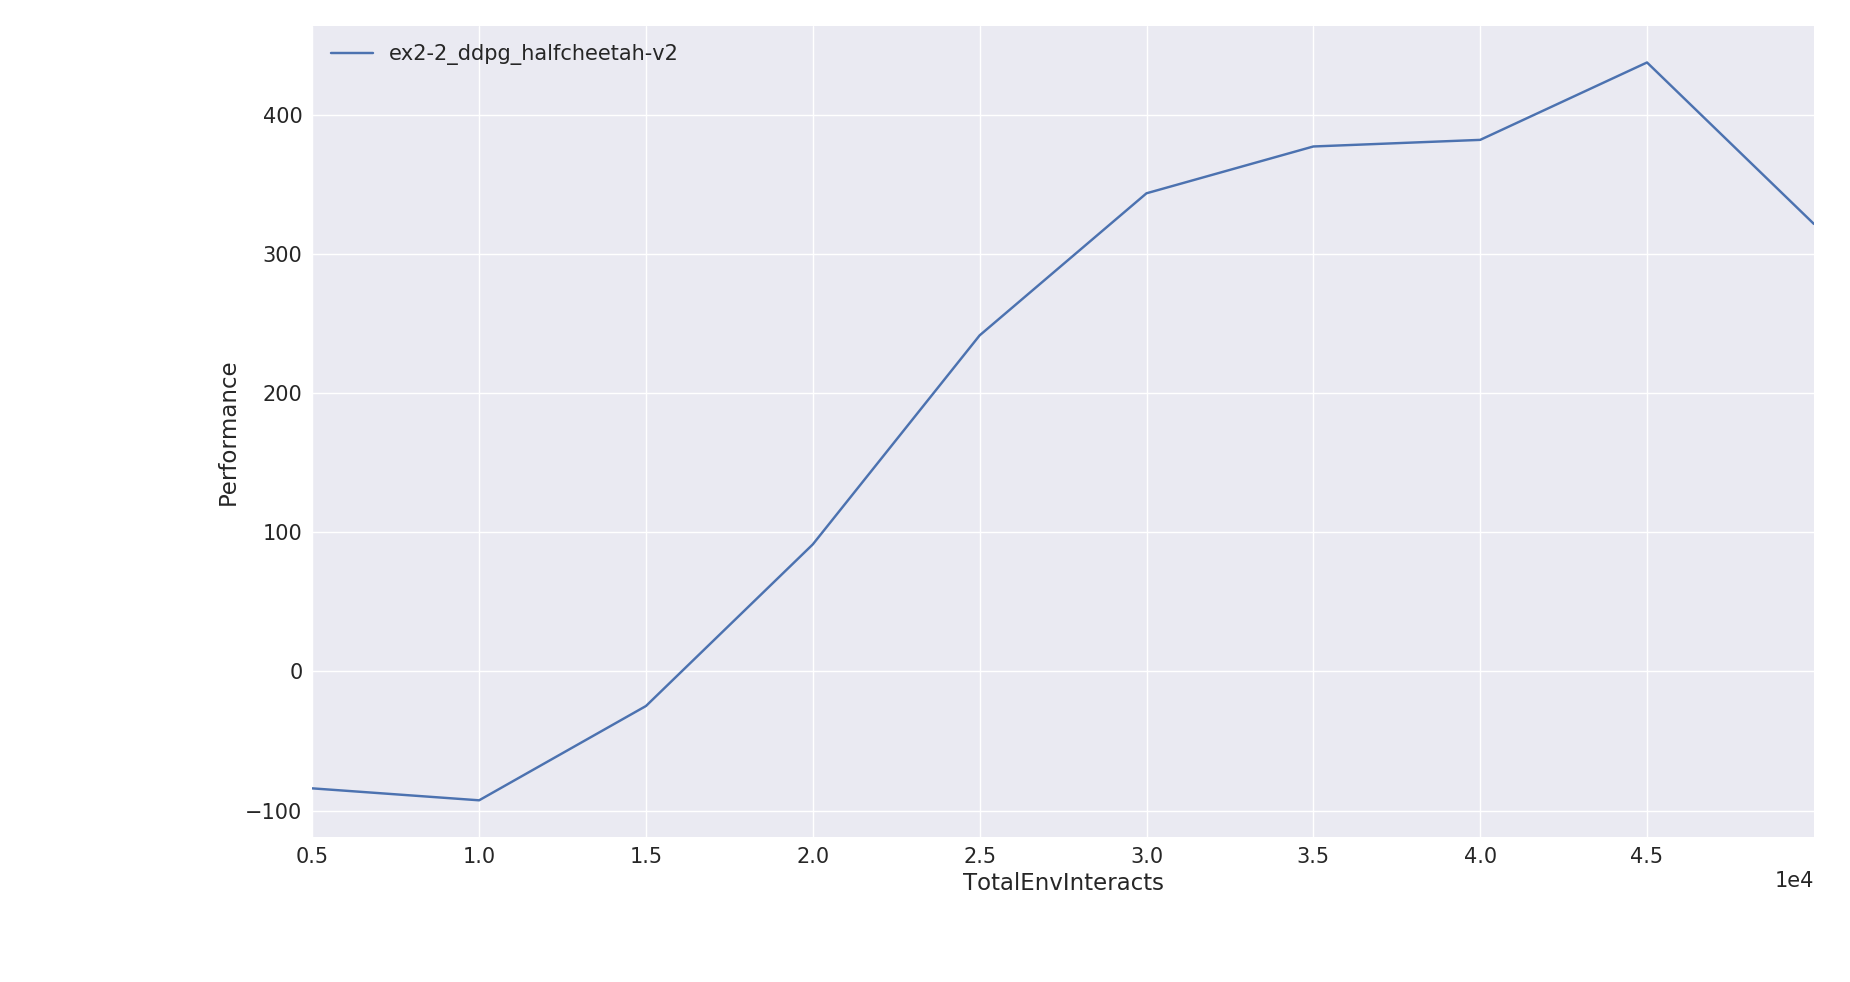
\includegraphics[width=0.32\textwidth]{../Img/spinningup_exercises/2_2/2_2_curve_s10.png}
        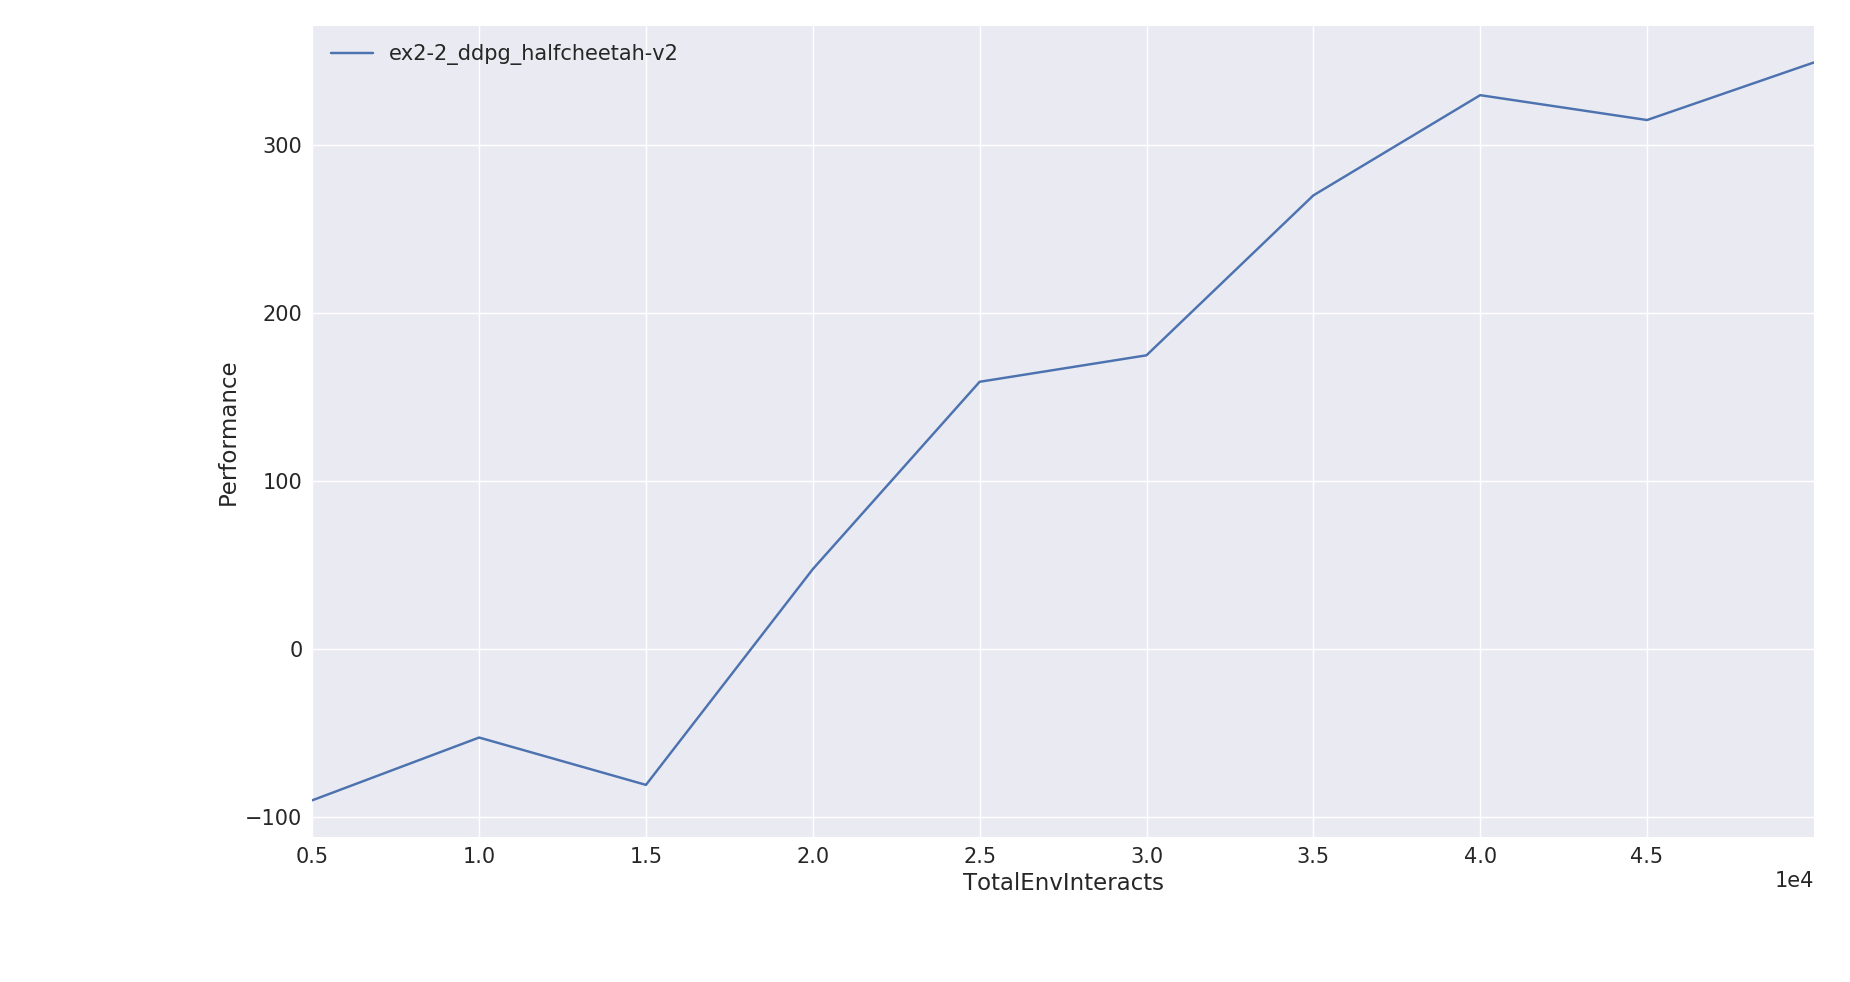
\includegraphics[width=0.32\textwidth]{../Img/spinningup_exercises/2_2/2_2_curve_s20.png}
    \end{figure}

    The curve of the code with bug and with different seeds are as follows:
    \begin{figure}[H]
        \centering
        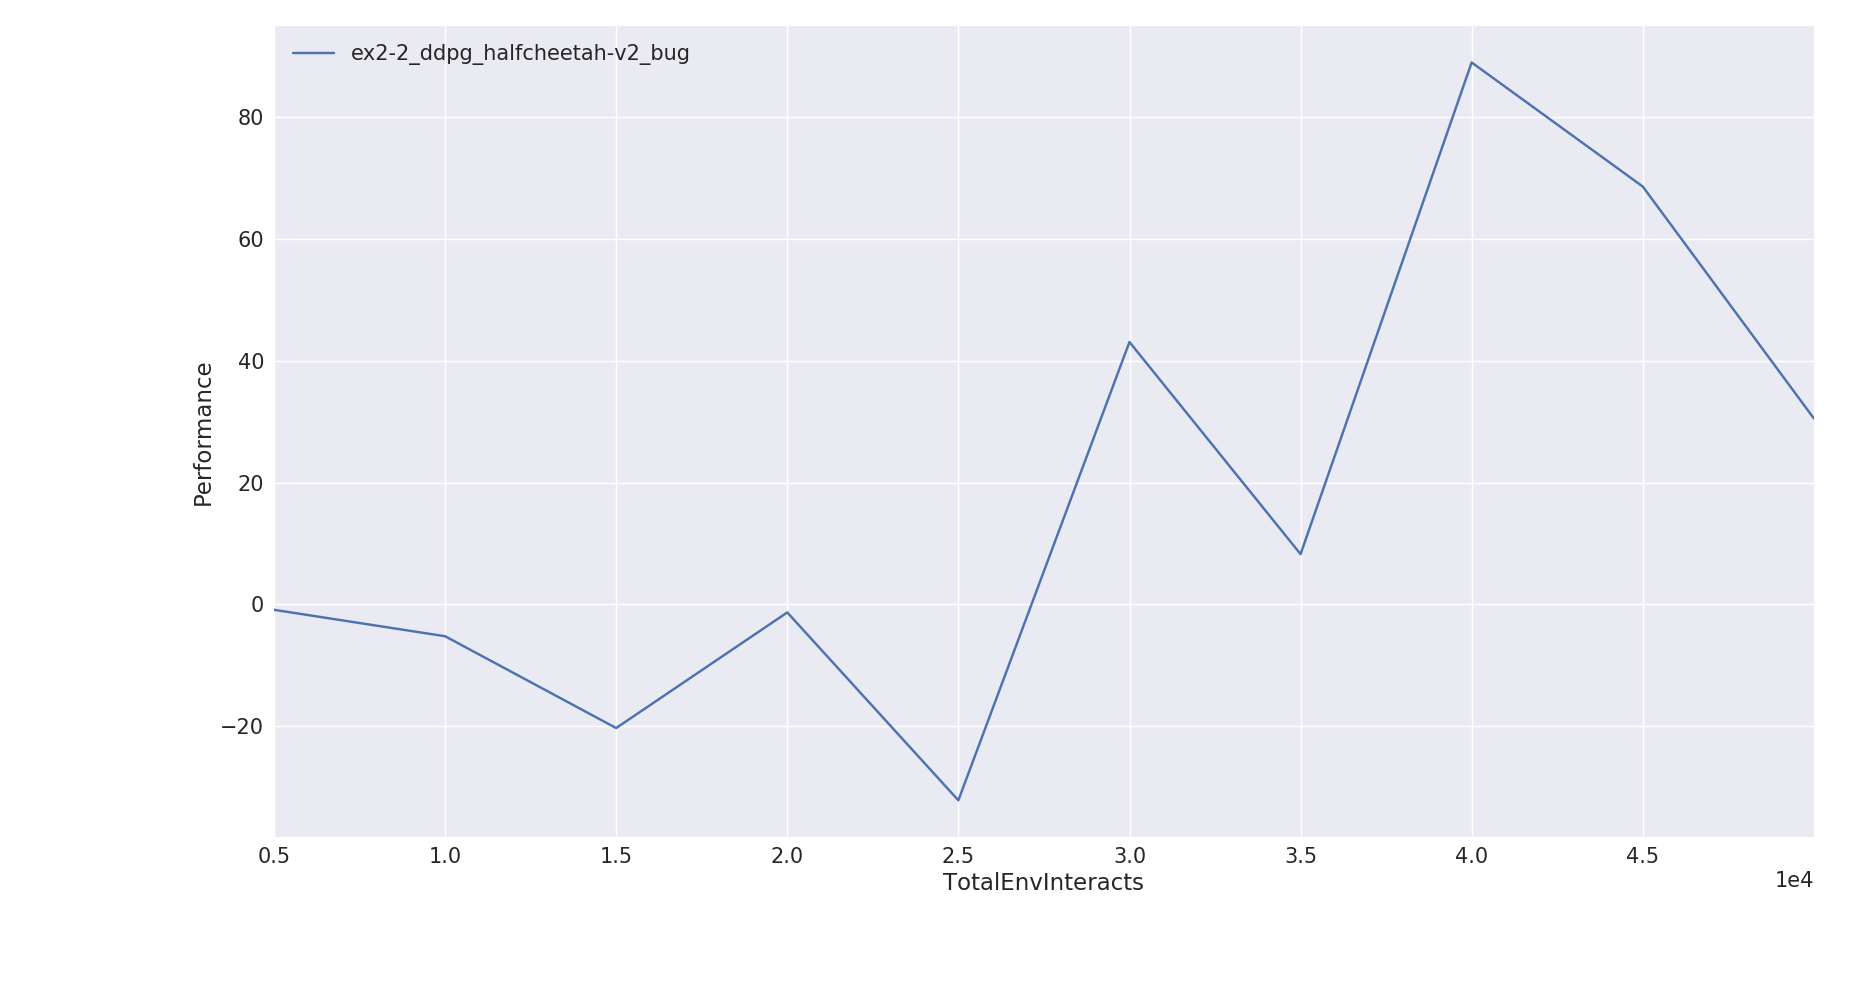
\includegraphics[width=0.32\textwidth]{../Img/spinningup_exercises/2_2/2_2_bug_curve_s0.png}
        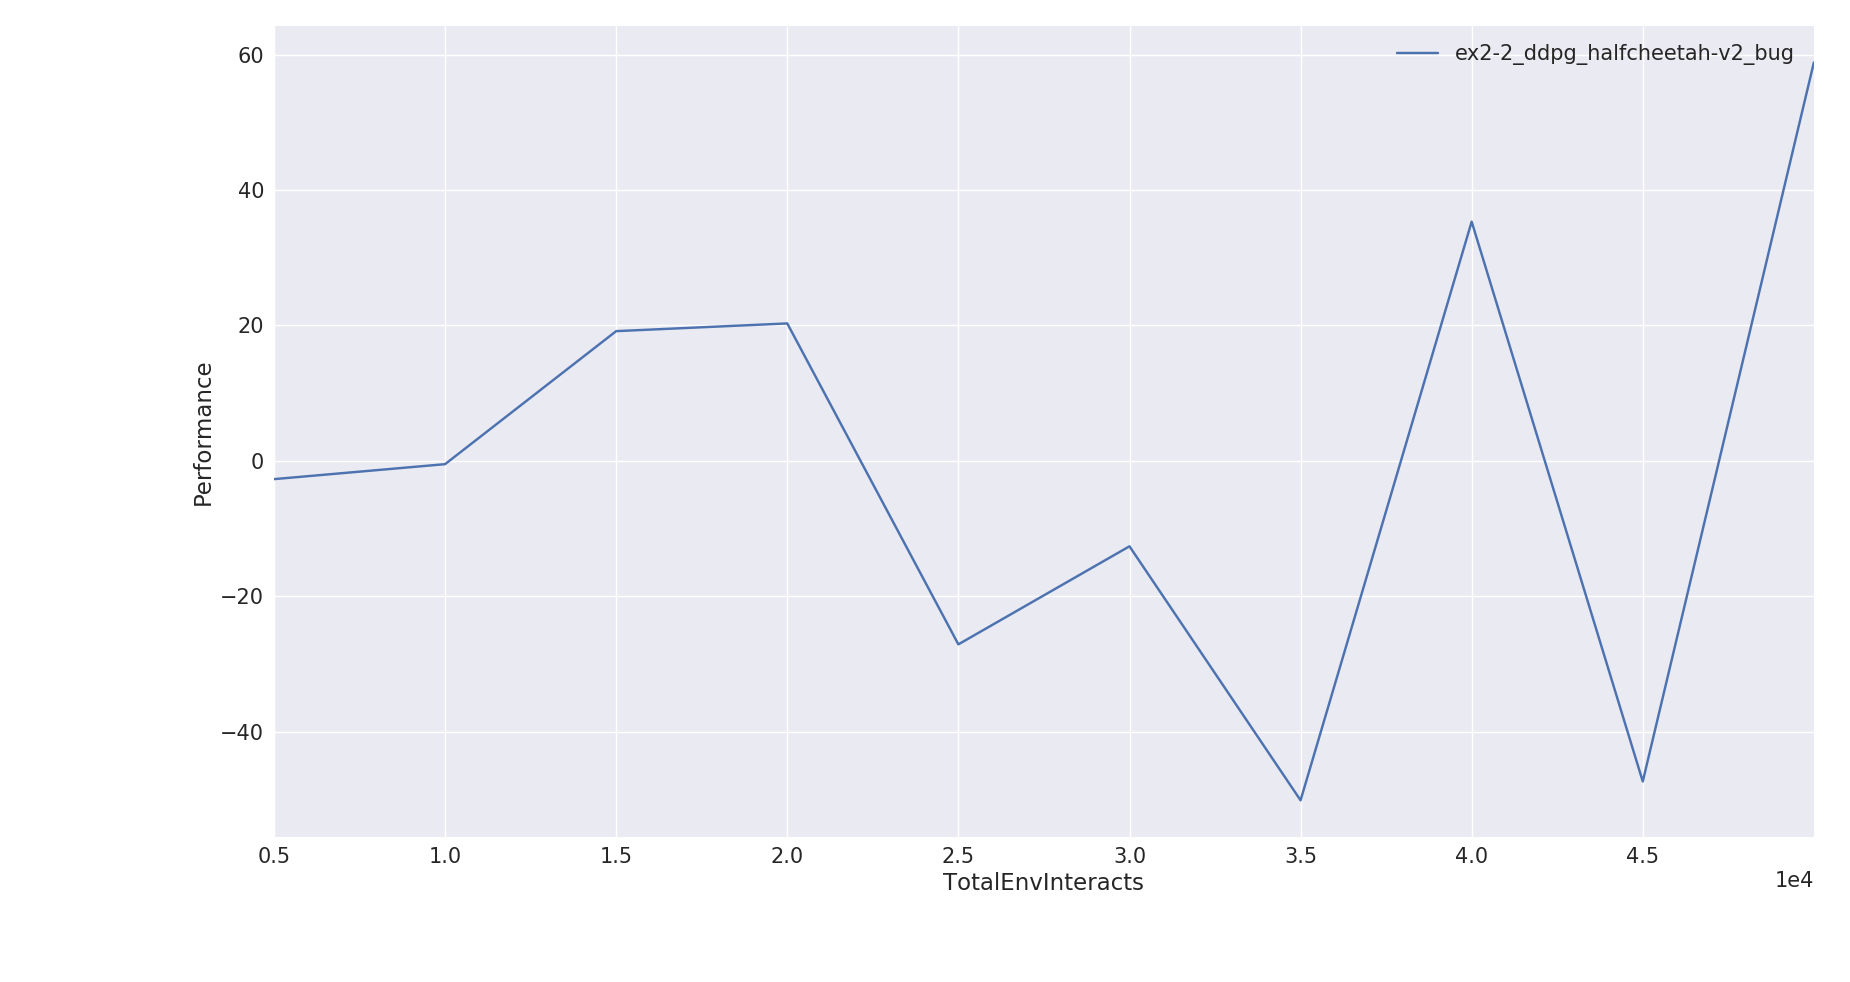
\includegraphics[width=0.32\textwidth]{../Img/spinningup_exercises/2_2/2_2_bug_curve_s10.png}
        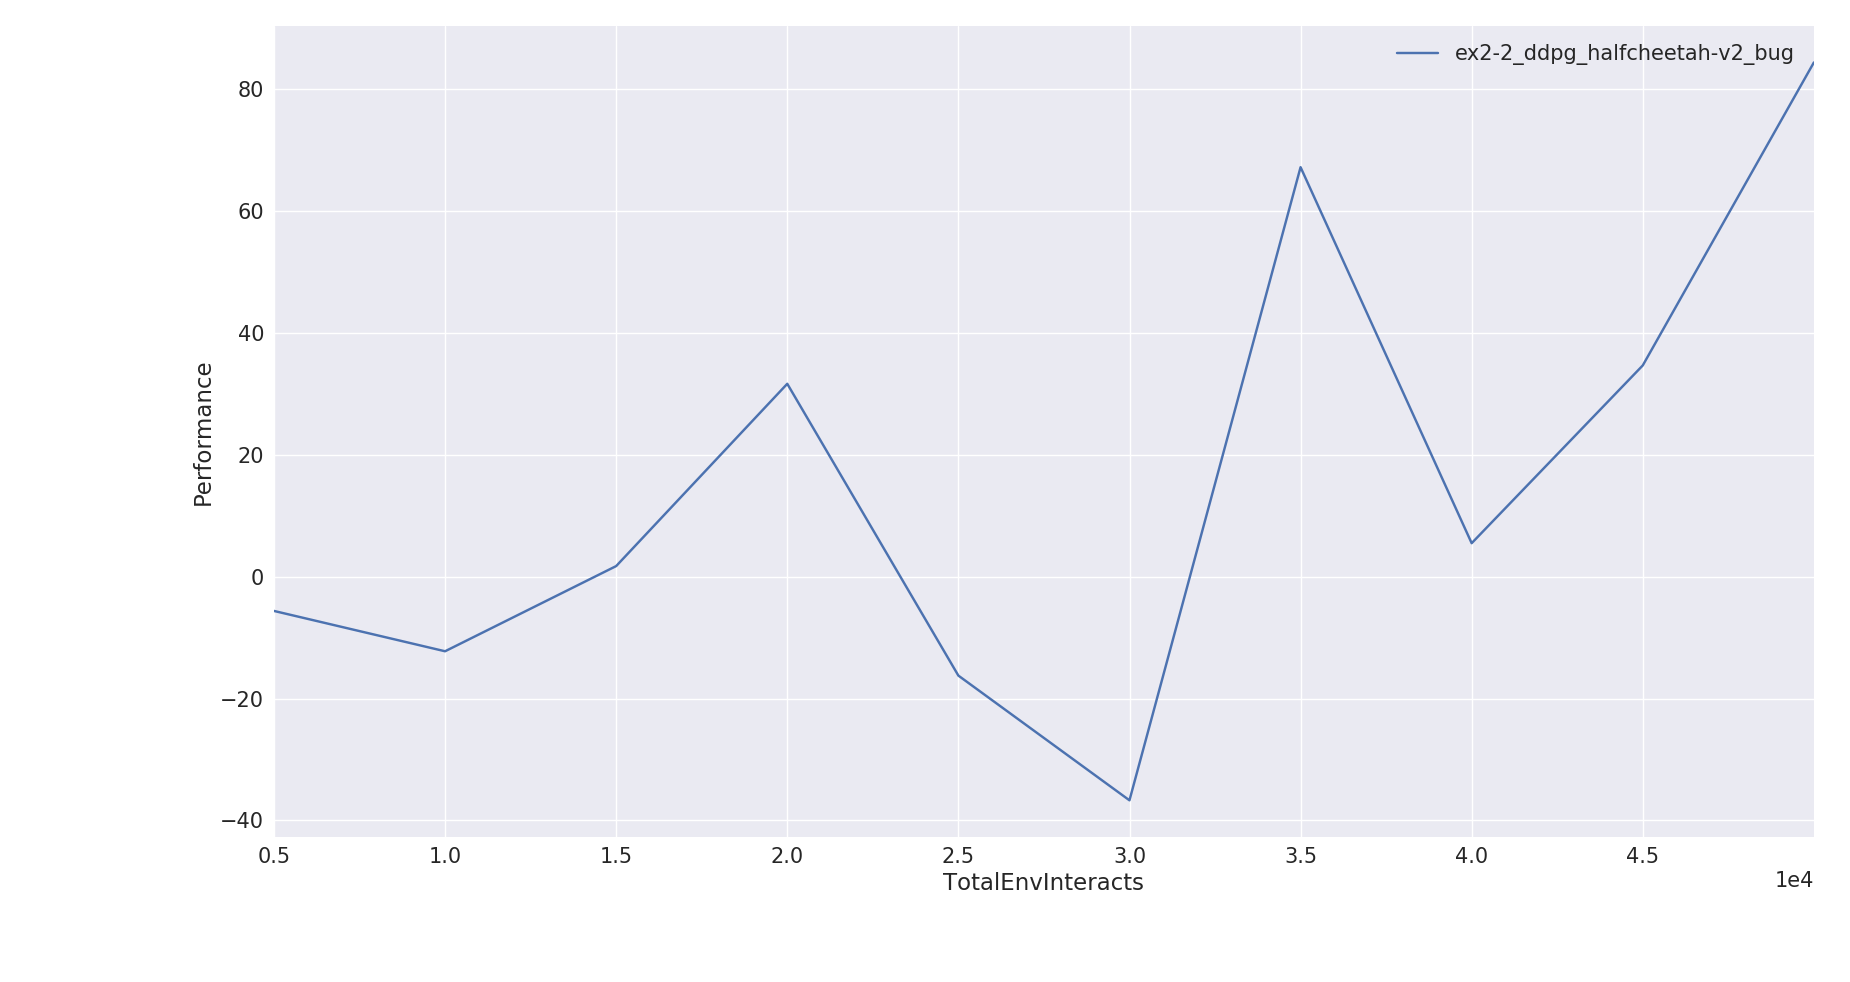
\includegraphics[width=0.32\textwidth]{../Img/spinningup_exercises/2_2/2_2_bug_curve_s20.png}
    \end{figure}

    The comparison between curve with and without bug, and their average and variance are as follows:
    \begin{figure}[H]
        \centering
        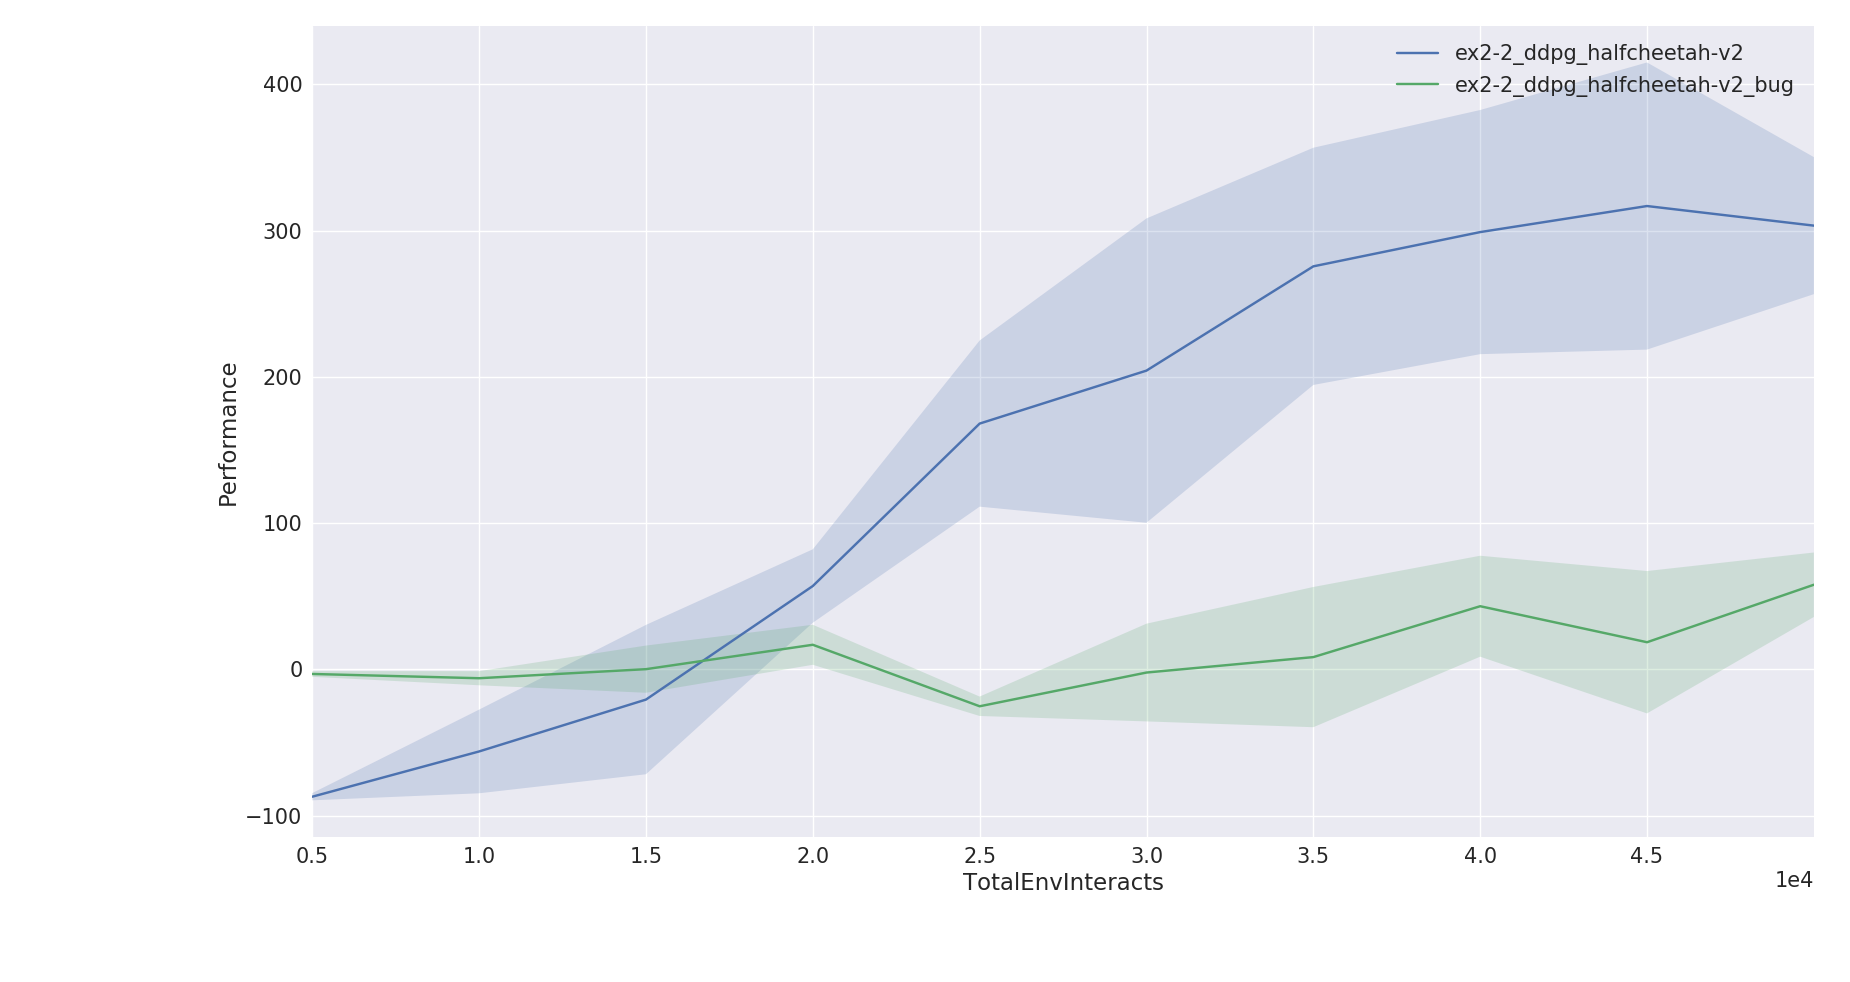
\includegraphics[width=\textwidth]{../Img/spinningup_exercises/2_2/2_2_curve_all.png}
    \end{figure}

    The code's bug is shown in the following figure:
    \begin{figure}[H]
        \centering
        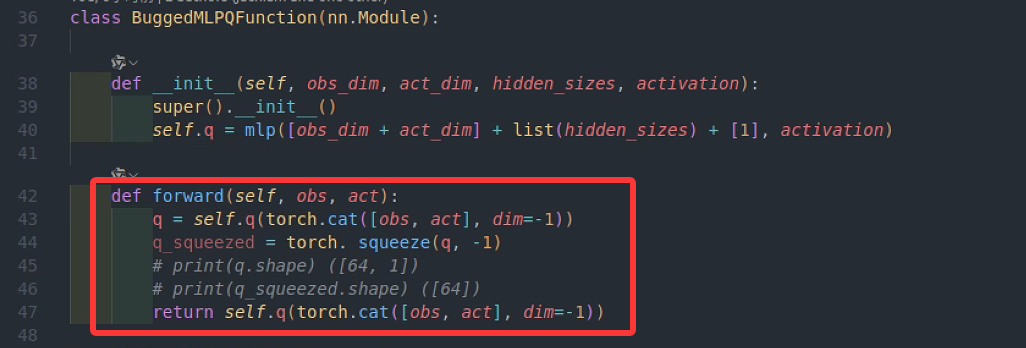
\includegraphics[width=\textwidth]{../Img/spinningup_exercises/2_2/2_2_mistake.png}
    \end{figure}


\end{itemize}



\end{homeworkProblem}

\newpage
\section{Part II: Performance Evaluation of Classical Bandit Algorithms}
You are required to use the Jupyter Notebook (Formerly known as the IPython Notebook) to submit your work.

\begin{itemize}
\item \textbf{Basic Setting} \\
We consider a time-slotted bandit system $(t=0,1,2, \ldots)$ with three arms. We denote the arm set as $\{1,2,3\}$. Pulling each arm $j(j \in\{1,2,3\})$ will obtain a reward $r_j$, which satisfies a Bernoulli distribution with mean $\theta_j\left(\operatorname{Bern}\left(\theta_j\right)\right)$, i.e.,
$$r_j= \begin{cases}1, & \text { w.p. } \theta_j \\ 0, & \text { w.p. } 1-\theta_j\end{cases}$$
where $\theta_j$ are parameters within $(0,1)$ for $j \in\{1,2,3\}$.

Now we run this bandit system for $N(N\gg 3)$ time slots. At each time slot $t$, we choose one and only one arm from these three arms, which we denote as $I(t) \in\{1,2,3\}$. Then we pull the arm $I(t)$ and obtain a reward $r_{I(t)}$. Our objective is to find an optimal policy to choose an arm $I(t)$ at each time slot $t$ such that the expectation of the aggregated reward is maximized, i.e.,
$$\max_{I(t), t=1, \ldots N} \mathbb{E}\left[\sum_{t=1}^N r_{r(t)}\right]$$
If we know the values of $\theta_j, j \in\{1,2,3\}$, this problem is trivial. Since $r_{T(t)} \sim \operatorname{Bern}\left(\theta_{I(t)}\right)$,
$$\mathbb{E}\left[\sum_{t=1}^N r_{I(t)}\right]=\sum_{t=1}^N \mathbb{E}\left[r_{I(t)}\right]=\sum_{t=1}^N \theta_{I(t)}$$
Let $I(t)=I^*=\underset{j \in\{1,2,3\}}{\arg \max } \theta_j$ for $t=1,2, \ldots, N$, then
$$\max _{I(t), t=1, \ldots, N} \mathbb{E}\left[\sum_{i=1}^N r_{I(t)}\right]=N \cdot \theta_{I^*}$$
However, in reality, we do not know the values of $\theta_j, j \in\{1,2,3\}$. We need to estimate the values $\theta_j$ via empirical samples, and then make the decisions at each time slot.
Next we introduce three classical bandit algorithms: $\epsilon$-greedy, UCB and Thompson sampling.

\item \textbf{Bandit Algorithms} \\
1. $\epsilon$-greedy Algorithm $(0 \leq \epsilon \leq 1)$
\begin{algorithm}[h]
\caption{$\epsilon$-greedy Algorithm}
\textbf{Initialize} $\hat{\theta}(j)\gets 0, \cnt(j)\gets 0, j \in \{1,2,3\}$
\begin{algorithmic}[1]
    \For {$t = 1,2,3,\ldots,N$}
        \State $I(t)\gets\begin{cases}
            \argmax\limits_{j\in\{1,2,3\}} \hat{\theta}_j, & \text{w.p. } 1-\epsilon \\
            \text{randomly choose from} \{1,2,3\}, & \text{w.p. } \epsilon
            \end{cases}$
        \State $\cnt(I(t))\gets \cnt(I(t)) + 1$
        \State $\hat{\theta}(I(t))\gets \hat{\theta}(I(t))+\frac{1}{\cnt(I(t))} \left[r_{I(t)}-\hat{\theta}(I(t))\right]$
    \EndFor
\end{algorithmic}
\end{algorithm}

2. UCB (Upper Confidence Bound) Algorithm \\
\begin{algorithm}[h]
\caption{UCB Algorithm}
\textbf{Initialize} $\hat{\theta}(j)\gets 0, \cnt(j)\gets 0, j \in \{1,2,3\}$
\begin{algorithmic}[1]
    \For {$t = 1,2,3$}
        \State $I(t)\gets t$
        \State $\cnt(I(t))\gets 1$
        \State $\hat{\theta}(I(t))\gets r_{I(t)}$
    \EndFor

    \For {$t = 4,\ldots,N$}
        \State $I(t)\gets\argmax\limits_{j\in\{1,2,3\}} \left(\hat{\theta}(j)+c\cdot \sqrt{\dfrac{2\log(t)}{\cnt(j)}} \right)$
        \State $\cnt(I(t))\gets \cnt(I(t)) + 1$
        \State $\hat{\theta}(I(t))\gets \hat{\theta}(I(t))+\frac{1}{\cnt(I(t))} \left[r_{I(t)}-\hat{\theta}(I(t))\right]$
    \EndFor
\end{algorithmic}
\end{algorithm}
\textbf{Note}: $c$ is a positive constant with a default value of 1.

3. Thompson sampling (TS) Algorithm \\
Recall that $\theta_j, j\in\{1, 2, 3\}$, are unknown parameters over (0, 1). From the Bayesian perspective, we assume their priors are Beta distributions with given parameters $(\alpha_j, \beta_j)$.
\begin{algorithm}[h]
\caption{TS Algorithm}
\textbf{Initialize} Beta parameter $(\alpha_j,\beta_j), j \in \{1,2,3\}$
\begin{algorithmic}[1]
    \For {$t = 1,2,3,\ldots,N$}
        \State \# Sample method
        \For {$j \in \{1,2,3\}$}
            \State Sample $\hat{\theta}(j) \sim \text{Beta}(\alpha_j, \beta_j)$
        \EndFor
        \State \# Select and pull the arm
        \State $I(t)\gets\argmax\limits_{j\in\{1,2,3\}} \hat{\theta}(j)$
        \State \# Update the distribution
        \State $\alpha_{I(t)}\gets \alpha_{I(t)} + r_{I(t)}$
        \State $\beta_{I(t)}\gets \beta_{I(t)} + 1 - r_{I(t)}$
    \EndFor
\end{algorithmic}
\end{algorithm}

\item \textbf{Simulation} \\
(1) Now suppose we obtain the Bernoulli distribution parameters from an oracle, which are shown in the following table below. Choose $N=10000$ and compute the theoretically maximized expectation of aggregate rewards over $N$ time slots. We call it the oracle value. Note that these parameters $\theta_j, j=1,2,3$ and oracle values are unknown to all bandit algorithms.
\begin{center}
\begin{tabular}{|c|c|c|c|}
    \hline $\operatorname{Arm} j$ & 1 & 2 & 3 \\
    \hline$\theta_j$ & 0.9 & 0.8 & 0.7 \\
    \hline
\end{tabular}
\end{center}

(2) Implement classical bandit algorithms with following settings: \\
- $N=5000$ \\
- $\epsilon$-greedy with $\epsilon=0.1,0.5,0.9$. \\
- UCB with $c=1,5,10$. \\
- Thompson Sampling with \\
$\left\{\left(\alpha_1, \beta_1\right)=(1,1),\left(\alpha_2, \beta_2\right)=(1,1),\left(\alpha_3, \beta_3\right)=(1,1)\right\}$ and \\
$\left\{\left(\alpha_1, \beta_1\right)=(601,401),\left(\alpha_2, \beta_2\right)=(401,601),\left(\alpha_3, \beta_3\right)=(2,3)\right\}$ \\
- Gradient bandit with baseline $b=0,0.8,5,20$. \\
- Parameterized gradient bandit with constant parameter $\beta=0.2,1,2,5$ \\
- Parameterized gradient bandit with time-varying parameters (you need to design a time-varying rule)

(3) Each experiment lasts for $N=5000$ turns, and we rum each experiment 1000 times. Results are averaged over these 1000 independent rums.

(4) Please report three performance metrics \\
- The total regret accumulated over the experiment. \\
- The regret as a function of time. \\
- The percentage of plays in which the optimal arm is pulled.

(5) Compute the gaps between the algorithm outputs and the oracle value. Compare the numerical results of $\epsilon$-greedy, UCB, Thompson Sampling and gradient bandit. Which one is the best? Then discuss the impacts of $\epsilon, C$, and $\alpha_j, \beta_j, b$, and $\beta$ respectively.

(6) What is the role of baseline in gradient bandit algorithm? Show your answer with simulation result.

(7) Give your understanding of the exploration-exploitation trade-off in bandit algorithms.

(8) Give your understanding of the adoption of sublinear regret as the performance threshold between good bandit algorithms and bad bandit algorithms.

\end{itemize}

\solution

(1) Since each arm's parameter is oracled, so we just need to choose the arm with the largest parameter to have the maximum expectation of aggregate rewards over $N$ time slots.

Since $\theta_1 = 0.9, \theta_2 = 0.8, \theta_3 = 0.7$, so we choose arm 1 everytime.

i.e.
\begin{align*}
\forall t, I(t)=I^* &= \argmax\limits_{j\in\{1,2,3\}}\theta_j=1 \\
\hat{\theta}_{I(t)} &= \theta_1 = 0.9 \\
r_{I(t)} \sim \text{Bern}(\theta_{I(t)}) &\Rightarrow \mathbb{E}(r_{I(t)}) = \hat{\theta}_{I(t)}
\end{align*}
So the maximum expected value is
\begin{align*}
&\quad\ \max_{I(t),t=1,2,\cdots,N}\ \mathbb{E}\left[\sum_{t=1}^Nr_{I(t)}\right] \\
&= \max_{I(t),t=1,2,\cdots,N}\ \sum_{t=1}^N\mathbb{E}\left[r_{I(t)}\right] \\
&= N \cdot \hat{\theta}_{I(t)} \\&= 10000 \times 0.9 \\
&= 9000
\end{align*}
So above all, with the given oracle parameters, the maximum expected value is 9000.

(2), (3) The implementation codes are in the `hw4\_code.ipynb' file.

(4) 1. The epsilon-greedy algorithm
\begin{table}[h]
    \centering
    \begin{tabular}{c c c}
    \toprule
    parameter & Average Regret & Optimal Percentage \\
    \midrule
    $\epsilon=0.1$ & 54.35  & 92.48\% \\
    $\epsilon=0.5$ & 251.34 & 66.30\% \\
    $\epsilon=0.9$ & 449.43 & 39.95\% \\
    \bottomrule
\end{tabular}
\vspace{-0.5cm}
\end{table}

\newpage
The regret and optimal percentage for $\epsilon$-greedy algorithm as a function of time are shown in the following figures:
\begin{figure}[h]
    \centering
    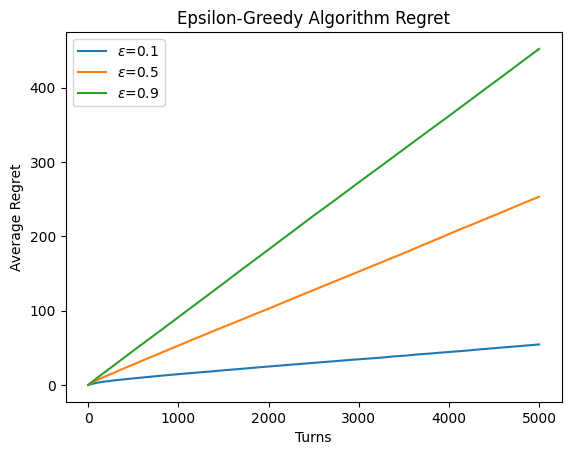
\includegraphics[width=0.49\textwidth]{./figure/epsilon_greedy_regret.png}
    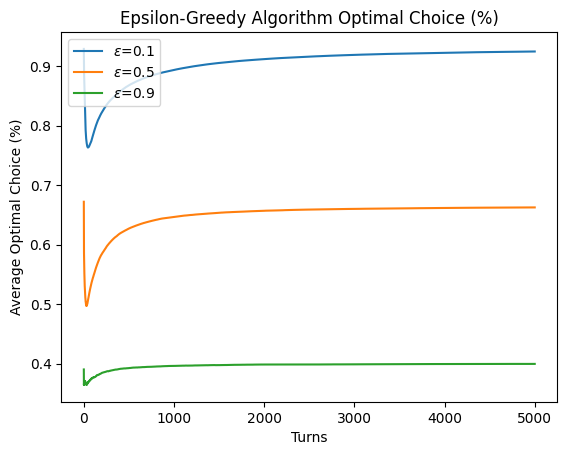
\includegraphics[width=0.49\textwidth]{./figure/epsilon_greedy_optimal.png}
\end{figure}

2. The UCB algorithm
\begin{table}[h]
    \centering
    \begin{tabular}{c c c}
    \toprule
    parameter & Average Regret & Optimal Percentage \\
    \midrule
    $c=1$  & 112.75 & 82.51\% \\
    $c=5$  & 372.65 & 47.20\% \\
    $c=10$ & 436.05 & 40.18\% \\
    \bottomrule
\end{tabular}
\end{table}

The regret and optimal percentage for UCB algorithm as a function of time are shown in the following figures:
\begin{figure}[h]
    \centering
    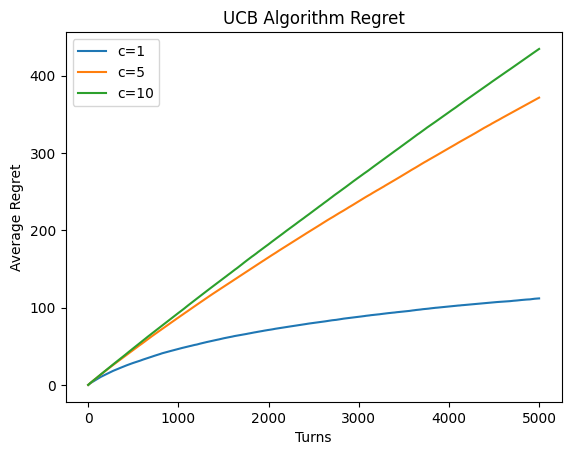
\includegraphics[width=0.49\textwidth]{./figure/UCB_regret.png}
    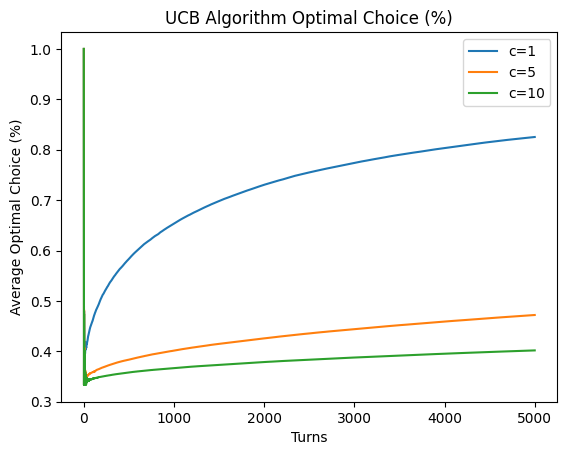
\includegraphics[width=0.49\textwidth]{./figure/UCB_optimal.png}
\end{figure}


3. The Thompson Sampling algorithm
\begin{table}[!htbp]
    \centering
    \begin{tabular}{c c c}
    \toprule
    parameter & Average Regret & Optimal Percentage \\
    \midrule
    $\alpha,\beta=[(1,1),(1,1),(1,1)]$         & 14.36  & 97.58\% \\
    $\alpha,\beta=[(601,401),(401,601),(2,3)]$ & 708.15 & 29.07\% \\
    \bottomrule
\end{tabular}
\end{table}

\newpage
\begin{figure}[h]
    \centering
    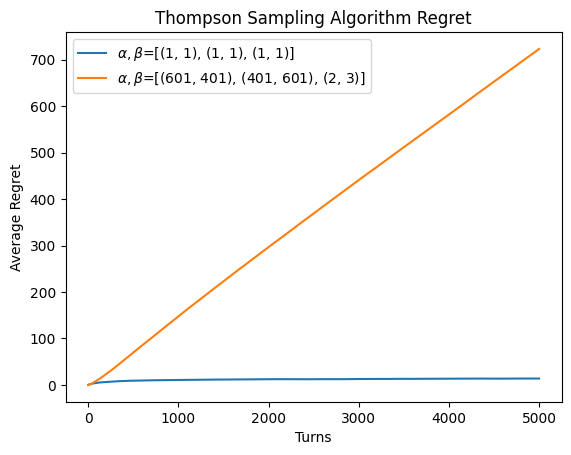
\includegraphics[width=0.49\textwidth]{./figure/TS_regret.png}
    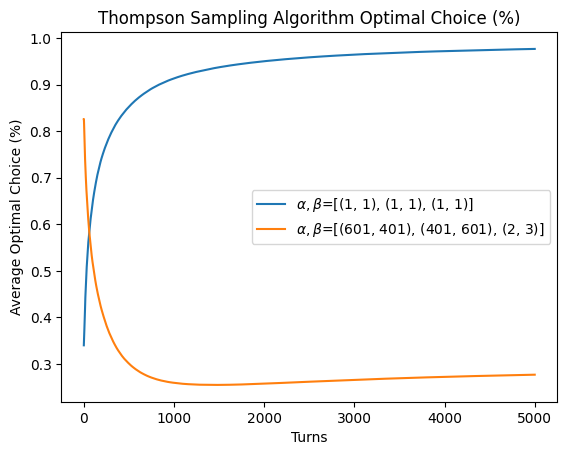
\includegraphics[width=0.49\textwidth]{./figure/TS_optimal.png}
\end{figure}

4. The Gradient Bandit algorithm \\
The step size is set to be $\alpha=0.1$. For the time-varient case, to have a smooth varying, set $\beta_0=0.1, \beta_T=10$:
$$\beta(t) = \beta_0 + \left( \frac{\log\left(1 + 9 \cdot \frac{t}{T} \right)}{\log(10)} \right) \cdot (\beta_T - \beta_0) = 0.1 + \left( \frac{\log\left(1 + 9 \cdot \frac{t}{T} \right)}{\log(10)} \right) \cdot (10 - 0.1)$$
And the baseline is set to be $B_t=\bar{R}_t$ is $b=-1$, otherwise it is set to be $B_t=b$.
\begin{table}[h]
    \centering
    \begin{tabular}{c c c}
    \toprule
    parameter & Average Regret & Optimal Percentage \\
    \midrule
    $b=0$   & 71.36  & 88.72\% \\
    $b=0.8$ & 50.37  & 92.72\% \\
    $b=5$   & 381.22 & 44.73\% \\
    $b=20$  & 490.65 & 33.18\% \\
    \midrule
    $\beta=0.2$ & 176.42 & 74.77\% \\
    $\beta=1$   & 49.97  & 92.60\% \\
    $\beta=2$   & 30.06  & 95.67\% \\
    $\beta=5$   & 16.57  & 97.55\% \\
    \midrule
    time-varying & 19.22 & 97.22\% \\
    \bottomrule
\end{tabular}
\vspace{-0.5cm}
\end{table}

\begin{figure}[!htbp]
    \centering
    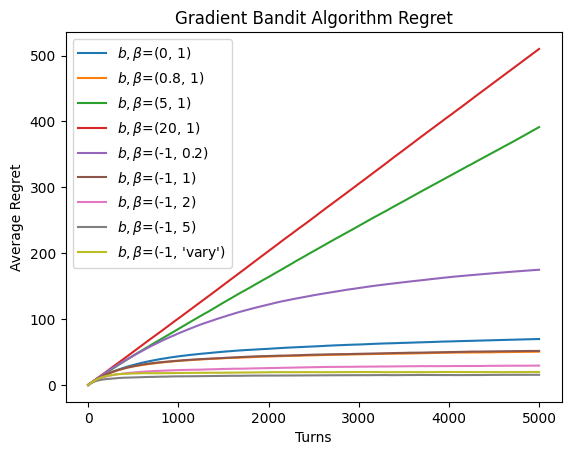
\includegraphics[width=0.49\textwidth]{./figure/gradient_bandit_regret.png}
    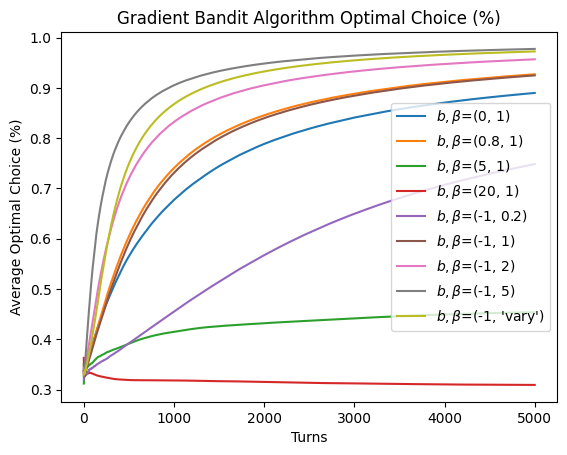
\includegraphics[width=0.49\textwidth]{./figure/gradient_bandit_optimal.png}
\end{figure}
\newpage

(5) The gap's comparison between the algorithms with different parameters is as follows:
\begin{table}[!htbp]
    \centering
    \colorbox{orange}{best}\ \colorbox{cyan}{second best} \\
    \begin{tabular}{c|c|c}
    \toprule
    \textbf{Algorithm} & \textbf{Parameter} & \textbf{Gap} \\
    \midrule
    \multirow{3}{*}{\centering $\epsilon$-Greedy}   & $\epsilon=0.1$ & 54.35  \\
                                                    & $\epsilon=0.5$ & 251.34 \\
                                                    & $\epsilon=0.9$ & 449.43 \\
    \midrule
    \multirow{3}{*}{\centering UCB} & $c=1$  & 112.75 \\
                                    & $c=5$  & 372.65 \\
                                    & $c=10$ & 436.05 \\
    \midrule
    \multirow{2}{*}{\centering TS}  & $\alpha,\beta=[(1,1),(1,1),(1,1)]$         & \cellcolor{orange}{14.36}  \\
                                    & $\alpha,\beta=[(601,401),(401,601),(2,3)]$ & 708.15 \\
    \midrule
    \multirow{10}{*}{\centering Gradient}   & $b=0$   & 71.36  \\
                                            & $b=0.8$ & 50.37  \\
                                            & $b=5$   & 381.22 \\
                                            & $b=20$  & 490.65 \\
    \cline{2-3}
    & $\beta=0.2$ & 176.42 \\
    & $\beta=1$   & 49.97  \\
    & $\beta=2$   & 30.06  \\
    & $\beta=5$   & \cellcolor{cyan}{16.57} \\
    \cline{2-3}
    & time-varying & 19.22 \\
    \bottomrule
    \end{tabular}
\end{table}

Comparing all rewards among the experiments we have done, we could find that the Thompson Sampling algorithm with parameter $\alpha,\beta=[(1,1),(1,1),(1,1)]$ is the best one, and gradient bandit algorithm with parameter $\beta=5$ is the second best one.

Then we can discuss the impacts of $\epsilon$, $c$, and $\alpha_{j}$, $\beta_{j}$, $b$, $\beta$ respectively.
\begin{itemize}
\item $\epsilon$-greedy algorithm \\
We have a parameter $\epsilon$, in our experiments, lower $\epsilon$ has a lower regret, however, it is still linear to the time.

\item the UCB algorithm \\
We choose the arm by the metric $\hat{\theta}(j)+c\cdot \sqrt{\dfrac{2\log(t)}{\cnt(j)}}$. In our experiments, we could find that the regret of the UCB algorithm with $c=1$ is the lowest. And the regret is sublinear to the time. Larger $c$ has a higher regret, and the regret looks like linear to the time when $c=5,10$.

\item the Thompson Sampling algorithm \\
In the Beta-Bernoulli Thompson Sampling algorithm, we have a parameter $\alpha$ and $\beta$ to decide $\hat{\theta}_j$ as it $\sim \Beta(\alpha,\beta)$, in our experiences, we could discover that $\alpha,\beta=[(1,1),(1,1),(1,1)]$ is the best one. This is because the prior brief is closer to the true distribution of the reward, and it is not in a wrong direction. $\alpha,\beta=[(601,401),(401,601),(2,3)]$ could be regarded as doing some of the experiments, but the experiment is in a wrong distribution with the oracle distribution, so a worse prior lead to a worse performance.

\item the Gradient Bandit algorithm \\
The motivation of introducting baseline in the policy gradient algorithm is mainly used to reduce variance and accelerate convergence to make the algorithm more stable. The parameter $\beta$ adjust the weights for the perference of the arm.

In ours experiments, baseline $b=0.8$ have a better performance all $b$s. This is because $b=0.8$ is closer to the best arm's oracle distribution $\theta_1=0.9$, so it has a better performance. And larger $\beta$ means more important to the perference of the arm so $\beta=5$ has a better performance. And in theoretically, $\beta$ should be small at beginning for exploration, and be larger for exploitation latter. However, in our experiments, the time-varying $\beta$ is worse than $\beta=5$. This may because the time-varying function is not well selected.
\end{itemize}

(6) The baseline in the gradient bandit algorithm is a reference point for the reward. It is used to reduce the variance of the reward and make the algorithm more stable. We can test the performance of the gradient bandit algorithm with different baseline and different $\beta$. $b=-1$ representing the baseline is the average reward $\bar{R}_t$.

\begin{table}[h]
    \centering
    \colorbox{orange}{best}\ \colorbox{cyan}{second best} \\
    \begin{tabular}{c c c}
    \toprule
    parameter & Average Regret & Optimal Percentage \\
    \midrule
    $b=-1, \beta=1$ & 51.38 & 92.57\% \\
    $b=0,  \beta=1$ & 73.54 & 88.41\% \\
    $b=1,  \beta=1$ & 50.44 & 92.65\% \\
    \midrule
    $b=-1, \beta=2$ & 29.04 & 95.66\% \\
    $b=0,  \beta=2$ & 76.34 & 86.75\% \\
    $b=1,  \beta=2$ & 30.16 & 95.75\% \\
    \midrule
    $b=-1, \beta=5$ & \cellcolor{orange}{16.07}  & 97.57\% \\
    $b=0,  \beta=5$ & 150.11 & 73.57\% \\
    $b=1,  \beta=5$ & \cellcolor{cyan}{16.59}  & 97.33\% \\
    \bottomrule
\end{tabular}
\vspace{-0.5cm}
\end{table}

\begin{figure}[!htbp]
    \centering
    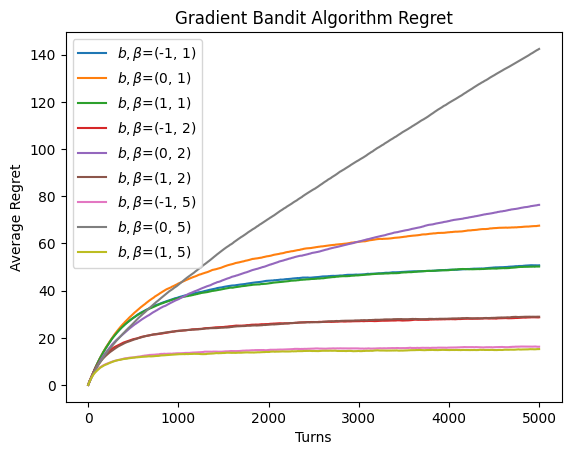
\includegraphics[width=0.49\textwidth]{./figure/gradient_bandit_baseline_regret.png}
    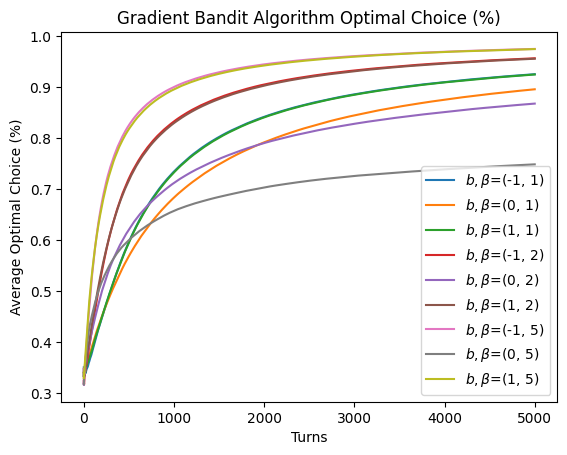
\includegraphics[width=0.49\textwidth]{./figure/gradient_bandit_baseline_optimal.png}
    \vspace{-0.5cm}
\end{figure}

And we can see that $\beta$ is the most significant parameter. Setting the baseline to be the average reward $\bar{R}_t$ has a better performance in ours experiments. If the baseline set not suitable, even a better $\beta$ could lead to a worse performance. For example, in ours experiment $b=0, \beta=5$ has a much larger average regret. And with baseline $B_t=\bar{R}_t, \beta=5$ has a much better performance. $b=0$ means without baseline, and we can see that in all settings of $\beta$, $b=0$, i.e. without baseline always has the highest regret.

(7) Exploration-Exploitation is a basic and popular topic in Reinforcement Learning. And it is also a very important topic in the bandit algorithm. At the beginning of playing with the bandit, we know nothing about the bandit. So we have to explore the bandit, gaining data from the previous decisions and feedbacks. Then after getting some information about the bandit, we can exploit them.

However, there must have a trade-off between exploration and exploitation. That is we have no idea how many times to explore, and when to start to exploit. If we always explore, we will never exploit to obtain better reward. And if we always exploit, we do not explore, and we may miss the best decision, go along the wrong way further and further. So we need to find a balance between exploration and exploitation. And this is the exploration-exploitation trade-off.
\begin{itemize}
\item $\epsilon$-greedy algorithm \\
We have a parameter $\epsilon$ to decide the probability of exploration and exploitation. If we set $\epsilon$ to be a small value, we will have a high probability to exploit the best arm we have found. And we will have a low probability to explore other arms. If we set $\epsilon$ to be a large value, we will have a high probability to explore other arms. And we will have a low probability to exploit the best arm we have found. So theoretically, the most suitable $\epsilon$ is time-varying: a larger value at the beginnig, and gradually decrease to a small value.

\item the UCB algorithm \\
We choose the arm by the metric $\hat{\theta}(j)+c\cdot \sqrt{\frac{2\log(t)}{\cnt(j)}}$. Where $\hat{\theta}(j)$ could be regard as exploitation, and $c\cdot \sqrt{\frac{2\log(t)}{\cnt(j)}}$ could be regard as exploration.

As for $c$, it is the parameter the decribe the degree of exploration. As $c$ increase, It turns to be more likely to explore. Correspondingly, as $c$ decrease, it more likely to exploitation.

So theoretically, the most suitable $c$ is time-varying: a larger value at the beginnig, and gradually decrease to a small value.

\item the Thompson Sampling algorithm \\
In the Beta-Bernoulli Thompson Sampling algorithm, we have a parameter $\alpha$ and $\beta$ to decide $\hat{\theta}_j\sim \Beta(\alpha,\beta)$. The Thompson Sampling algorithm is somehow more like a Bayesian method. We have a prior belief of the distribution of the reward. And we update the belief according to the reward we get.

The initial parameters $\alpha$ and $\beta$ are the prior belief of the distribution of the reward. And we update the parameters according to the reward we get with the Beta-Binomial conjugate. If we set $\alpha_j$ and $\beta_j$ to be a small value, we can regard that the prior tests time are less. i.e. with less prior tests, also less exploration. If we set $\alpha_j$ and $\beta_j$ to be a large value, we can regard that the prior tests time are more. i.e. with more prior tests, also more exploration.

\item the Gradient Bandit algorithm \\
The parameter $\beta$ adjust the weights for the perference of the arm, smaller $\beta$ means more exploration, larger $\beta$ means more exploitation. In our experiments, we could find that the gradient bandit algorithm with $\beta=5$ is the best one. In a suitable range, larger $\beta$ has a better performance.

So theoretically, the most suitable $\beta$ is time-varying: a larger value at the beginnig, and gradually decrease to a small value.
\end{itemize}

(8) Intuitively, linear regret means that the algorithm failed to learn effectively: its average regret per step is a constant, instread of decreasing over time, indicating that the algorithm cannot improve decisions through historical experience.

But for sublinear regret, which means that $\lim\limits_{t\to+\infty}\dfrac{L_t}{t}=0$, where $L_t$ is the total regret at time $t$. Indicating that the average regret per step of the algorithm tends towards zero. The algorithms gradually learn to choose actions that are close to optimal, reflecting effective exploration and utilization of the environment.

Theoretically, it is proved that the asymptotic total regret's lower bound has
$$\lim_{t\to+\infty} L_t\geq \log t\sum_{a|\Delta_a>0}\dfrac{\Delta_a}{KL(\R^a\|\R^{a*})}$$
Which is a sublinear regret. So if a algorithm has a sublinear regret, it reach the theoretical asymptotic optimal, and it is a good algorithm.

\newpage

\end{document}